\documentclass[sigplan,10pt]{acmart}
\renewcommand\footnotetextcopyrightpermission[1]{}

\settopmatter{printfolios=true, printacmref=false}

\usepackage{tikz}
\usepackage{float}
\usepackage{amsmath}
\usepackage{xspace}
\usepackage{cleveref}
\usepackage{balance}
\usepackage{url}
\usepackage{siunitx}
\usepackage{comment}
\usepackage{enumitem}
\usepackage{listings}
\usepackage{minted}
\usepackage{tikz}
\usepackage{subcaption}
\usepackage{booktabs} % For formal tables

\newcommand*\circled[1]{\tikz[baseline=(char.base)]{
            \node[shape=circle,draw=black!80,line width=0.2mm,inner sep=0.1pt] (char) {#1};}}

\newcommand{\sys}{UbiBPF\xspace}
% \newcommand{\tech}{Userspace Offload\xspace}

\newcommand{\eg}{e.g.,\xspace}
\newcommand{\ie}{i.e.,\xspace}
\newcommand{\etc}{etc.\xspace}

% Cleveref formatting
\crefname{algocf}{algorithm}{algorithms}
\Crefname{algocf}{Algorithm}{Algorithms}
\crefformat{section}{\S#2#1#3}
\Crefformat{section}{Section~#2#1#3}
\crefformat{subsection}{\S#2#1#3}
\Crefformat{subsection}{Section~#2#1#3}
\crefformat{subsubsection}{\S#2#1#3}
\Crefformat{subsubsection}{Section~#2#1#3}
\crefformat{figure}{figure~#2#1#3}
\Crefformat{figure}{Figure~#2#1#3}


% Numbers
\newcommand{\numcases}{6\xspace}
\newcommand{\speedupAccel}{xxx\xspace}
\newcommand{\eBPFSlowdownAccel}{xxx\xspace}
\newcommand{\speedupMonitor}{xxx\xspace}


\newlength{\mintednumbersep}
\AtBeginDocument{%
  \sbox0{\tiny00}%
  \setlength\mintednumbersep{\parindent}%
  \addtolength\mintednumbersep{-\wd0}%
}

\setminted{linenos}
\setminted{xleftmargin=12pt} % what a hack.
\setminted{numbersep=\mintednumbersep}
\setminted{mathescape}
\setminted{fontsize=\footnotesize}


%fixup some random size things:
\widowpenalty=300
\clubpenalty=300

%%% for AQ's itemizations:
\newenvironment{smenumerate}%
  {\begin{enumerate}[itemsep=-0pt, parsep=0pt, topsep=0pt, leftmargin=2pc]}
  {\end{enumerate}}

\newenvironment{smitemize}%
  {\begin{list}{$\bullet$}%
    {\setlength{\parsep}{0pt}%
      \setlength{\topsep}{0pt}%
      \setlength{\leftmargin}{2pc}%
      \setlength{\itemsep}{1pt}}}
  {\end{list}}

  



\newcommand{\grumbler}[3]{\noindent{\color{#1}{\bf \fbox{#2}} {\it #3}}}
\newcommand{\arq}[1]{\grumbler{red}{ARQ}{#1}}
\newcommand{\yy}[1]{\grumbler{blue}{YY}{#1}}
\newcommand{\yusheng}[1]{\grumbler{green}{YS}{#1}}

\newcommand{\todo}[1]{\grumbler{olive}{todo}{#1}}


\title{\sys: Extending Everything, Everywhere, Safely, Efficiently, and Dynamically. All at Once.}
% anyauthor declaration will be ignored  when using 'pldi' option (for double blind review)
%

% \author{
%     {\rm Yusheng Zheng}\\ eunomia-bpf Community
%     \and
%     {\rm Tong Yu} \\ eunomia-bpf Community
%     \and
%     {\rm Yiwei Yang}\\ UC Santa Cruz
%     \and
%     {\rm Yanpeng Hu}\\ShanghaiTech University
%     \and
%     % {\rm XiaoZheng Lai}\\South China university of technology
%     % \and
%     {\rm Andrew Quinn}\\ UC Santa Cruz
% }

\author{Paper \#371}

\begin{document}


\begin{abstract}
Software system extensions are useful for system administrators to customize software for the needs of a deployed system and also for adding monitoring and observability logic to better understand a system’s behavior across the entire software stack.  We find that modern use cases demand four characteristics from an extension framework: (1) comprehensiveness, (2) dynamism, (3) safety, and (4) efficiency.  Recently, a thriving ecosystem has grown around the eBPF kernel extension framework, which promises near perfect comprehensiveness, dynamism, and safety.  However, while eBPF succeeds in the kernel, it has fails to provide an ideal extension solution due to its lack of both efficiency and expressive power for userspace extensions. This paper presents \sys{}, a new framework that extends the eBPF framework that addresses these challenges.  \sys{} maintains comparability with the current eBPF ecosystem and provides an efficient, yet safe, solution for userspace extensions through a mixture of dynamic binary instrumentation, eBPF bytecode verification, and hardware-based isolation.  We demonstrate the breadth of \sys{} on \numcases{} use-cases that improve security, monitor performance, improve performance, and explore configuration tradeoffs.
\end{abstract}




\maketitle
\section{Introduction}

System administrators extend their software systems to customize it for their needs.  These extensions may tailor the application for hardware or a particular workload, as exemplified by works that improve system performance through extensions~\cite{Ghigoff21, Zhong22}.  Extensions may also enable system observability, as exemplified by works that extend systems to improve security~\cite{Jia23} or monitor performance~\cite{Gregg19, shen2023network,Zhu23}.  

For example, consider a system administrator who aims to understand the role of low-level library and kernel behavior on the tail latency of a microservice application.  The administrator could use system extensions to inject monitoring code across their software stack.  They would track requests by injecting monitoring logic into the application, track synchronization primitives by injecting logic into dependent libraries (\eg the \texttt{go} runtime, \texttt{libc}), and track kernel structures by injecting logic into the kernel.  The extensions would communicate so that the administrator could associate synchronization and kernel behavior with individual requests.

Extensions are fundamentally different from traditional software.  First, extensions require \emph{comprehensiveness}, or the ability to  interact with all of a system's software layers.  Second, extensions require \emph{dynamism}, or the ability to be added to a running system, so that the user can add monitoring or tune customization on the actual hardware and workloads that their system encounters.  Third, extensions require \emph{safety}, or the assurance that a buggy extension does not crash the system and that a subverted application cannot circumvent any extensions.  Safety is especially important for security monitoring extensions and for scenarios where the extension writer is not the original software developer of the extended system.  Finally, extensions require \emph{efficiency}, or the ability to execute at near native speed. 

Alas, existing system extension frameworks do not meet these needs.  Most systems are not comprehensive, as they only allow extensions to userspace applications (\eg dynamic binary instrumentation tools~\cite{Luk05, Nethercote07, Bruening12}, \texttt{LD\_PRELOAD}-based solutions, \etc) or only allow extensions to the operating system (\eg Nooks~\cite{Swift03}, VINO~\cite{Seltzer96}, SPIN~\cite{Bershad95}, linux kernel modules, \etc).   Extended Berkeley Packet Filters (eBPFs) are \emph{almost} comprehensive; they allow a user to extend the logic of the kernel and userspace applications, with the caveat that userspace extensions cannot modify userspace behavior. 
%\yusheng{behavior -> execution?}\arq{behavior just meaning "actions", but slightly fancier wording}
eBPF is dynamic, since users can extend a running system.  eBPF is safe since it uses a bytecode verifier to ensure that extensions cannot crash the system and executes extensions in the kernel to ensure that extensions are isolated from subverted applications.  However, eBPF is \emph{not} efficient, since its isolation approach requires multiple context switches to execute a userspace extensions.  For use cases with frequently-executed application extensions, such as the microservice monitoring example, this context switching overhead is substantial and can even lead to incorrect conclusions about the cause of performance degradation.

This paper presents \sys, a new system for comprehensive, dynamic, safe, and efficient extensions.  \sys{} is based upon two design principles.  First, the system maintains compatibility with the eBPF ecosystem so that it can build on eBPF's widespread adoption.  Second, the system resolves the inefficiency of the eBPF ecosystem by executing userspace extensions in the execution context of the extended application without requiring kernel involvement.  %Following these design principles, \sys{} enables the microservice monitoring use case to accurately measure performance and identify bottlenecks.

% and efficient full system extensions by allowing developers to ubiquitously use eBPF across their entire system.  \sys is compatible with the existing eBPF ecosystem, which makes it easy for developers to adopt.  Namely, developers extend kernel logic by hooking \texttt{kprobe}s, \texttt{kretprobe}s, and (\texttt{syscall}) \texttt{tracepoint}s; and extend application logic by hooking \texttt{uprobe}s and \texttt{uretprobe}s.  \sys provides a shared memory interface that allow extensions to communicate, whether the extensions are across system layers (\ie userspace extension that shares data with a kernel extension) or across processes (\ie a userspace extension from one process sharing data with a userpsace extension for another process).  \sys ensures extension safety---applications cannot interfere with extensions---and efficiency---extensions impose low runtime overhead.  Thus, with \sys, the microservice developer's monitoring is efficient and accurately measures performance.

% \yusheng{\sys provides a shared memory interface and data structs, so that extensions can communicate or aggregation data between different process or between kernel space and user space. For example, The kernel kprobe eBPF program, which runs in the kernel,  can update a variable in share memory to notify the  uprobe eBPF program, which runs in userspace the fsync operation is completed; The SSL/TLS unencrypted traffic data between different process can be obtained by uprobe, and analysis metrics without sending them all to a centric agent.} 
%\yusheng{I think it may not be accurate to describe bpftime as "API compatible"? The compatible of bpftime is more like compatible with syscalls. From the bpf program side, we provide compatible with helpers(like the syscall id) and maps(like stl lib in cpp); for the tracing application like bpftrace, we emulate bpf syscall behavior in linux systems.}


Realizing \sys{}'s design principles requires overcoming three challenges.  First, \sys{} requires an eBPF ecosystem to execute eBPF extensions in userspace; the ecosystem must be feature compatible with the existing eBPF.  \sys{} solves this challenge with an ``extra layer of indirection'', a software layer that interposes on all requests made to eBPF and forwards them to \sys{}.  Second, \sys{} requires trap-free attachment to an arbitrary program to ensure that userspace extensions can execute without kernel involvement.  \sys{} solves this challenge by using binary rewriting~\cite{Dinesh20, Chamith17, WilliamsKing20, fridagum} to inject userspace extensions into an application.  Finally, executing userspace extensions in the extended application threatens the safety of \sys{}, since it complicates the use of the existing in-kernel eBPF bytecode verifier and breaks the isolation between extensions and applications.  \sys{} solves this challenge by using a userspace eBPF bytecode verifier~\cite{Gershuni19} to prevent a buggy extension from harming an application, and by adopting work on intra-process hardware memory protections~\cite{Vahldiek19, xie2022cetis}, to prevent a subverted application from circumventing an extension. 

% The key to empowering \sys's safety and efficiency is a new technique called \tech. \tech enables efficient userspace extensions by executing them directly in the context of the original application, similar to binary instrumentation~\cite{Luk05}.  \tech's key innovation  is its low-overhead load-time approach to ensuring isolation between applications and extensions that contrasts with the expensive heavyweight sandbox approach employed in prior work.  Namely, \tech reuses existing eBPF verifiers~\cite{Gershuni19, linuxverifier} to ensure that each extension does not interfere with the program that it extends (\eg an extension cannot cause a program to have a null-pointer exception). \tech employs recent hardware features (\ie control-flow enforcement technology and memory protection keys) to ensure that the original application cannot interfere with the extension.

We implement \sys{} on linux.  The implementation requires \emph{no changes} to the operating system, since it is implemented entirely in the existing eBPF ecosystem.  Thus, a user can write extension against the well-known eBPF ecosystem, execute them on a regular linux kernel, and still benefit from \sys{}'s enhanced comprehensiveness and efficiency.

We illustrate the generality of \sys by using it in \numcases use-cases (\cref{sec:use_cases}).  The use-cases explore design tradeoffs, improve security, monitor performance, and improve system performance.  In particular, we use \sys to monitor a microservice application, create new durability configurations in Redis, cache meta data operations in FUSE, implement a ssl-supporting distributed tracing tool, monitor system calls for performance monitoring, and enhance Nginx's security.

We evaluate \sys's performance on the aforementioned \numcases use-cases.  We find that: \sys improves the throughput of profiling microservices by a factor of 1.5 compared to eBPF.  \sys{} enables a redis durability configuration that is 5 orders of magnitude more durable than the existing default setting, but only decreases throughput by ~10\%.  \sys enables FUSE caching that accelerates operations by orders of magnitude.  \sys{} reduces the overhead of SSL traffic monitoring by a factor of 1.67 compared to native eBPF.  And, \sys offers configurations that prevent monitoring overhead from affecting unmonitored processes, whereas eBPF is unable to do so.  We also use microbenchmarks to illustrate the key features that enable \sys's performance advantages and show \sys's compatibility with eBPF.

In sum, our contributions are:
\begin{smitemize}
\item An examination of system extension use-cases and the distillation of four design goals: comprehensiveness, dynamism, safety, and efficiency. 
\item \sys, a comprehensive, dynamic, safe, and efficient extension framework that maintains comparability with the eBPF ecosystem and adds efficiency by executing userspace extensions without kernel involvement.
\item An evaluation of a \sys showing that it is useful in \numcases use-cases and significantly more efficient than state-of-the-art alternatives.
\end{smitemize}

The rest of the paper is as follows.   We motivate system extensions and derive design goals (\cref{sec:motivation}).  We elaborate on the design principles and challenges in building the system (\cref{sec:challenges}).  Then, we discuss \sys's design (\cref{sec:design}) and implementation (\cref{sec:implementation}).  We discuss the \numcases use-cases (\cref{sec:use_cases}).   Next, we describe our evaluation (\cref{sec:evaluation}), related work (\cref{sec:related_work}), and conclude (\cref{sec:conclusion}).

\section{Motivation and Goals}\label{sec:motivation}

System extensions allow a user to enhance or augment software without modifying its source code.  Users turn to extensions to either \emph{customize} software for a particular workload and hardware configuration or to \emph{observe} software behavior to understand and diagnose issues.   Extension users are technical; they are comfortable writing code to modify a system's behavior.  However, extension users are \emph{not} the original developers of the extended system.  Consequently, extension users are not comfortable directly modifying their application's source code for fear of breaking it.  % They may third-parties, who release software patches for customization and observation.  But, the administrator is dubious of the correctness of third-party patches that have not been accepted into the mainline system.  

In the rest of this section, we discusses two use-cases that illustrate how system extensions solve the challenges faced by system administrators (\cref{sec:motivation:examples}).  We then derive four design constraints that an extension framework must satisfy for these use-cases (\cref{sec:motivation:constraints}).  Finally, we identify the limitations of existing extension frameworks (\cref{sec:motivation:limitations}).

\subsection{Extension Use-Cases}\label{sec:motivation:examples}

This section elaborates on two use-cases, one for observability and the other for customization.

\paragraph{Observability with DeepFlow}

Consider a system administrator who manages a microservice application.  The microservice uses logic across numerous software layers (application code, language runtime, and the operating system).  To understand system performance, the administrator needs to track application behavior across software layers. DeepFlow~\cite{shen2023network} is an extension-based approach to microservice monitoring that provides monitoring across software layers.  DeepFlow extends the operating system to track its networking logic and capture low-level metrics, such as TCP re-transmissions, that effect system performance.  DeepFlow also extends userspace applications and libraries to capture data not available in the kernel, such as coroutine IDs and message payloads before TLS encryption.  Finally, DeepFlow includes a userspace program that combines the monitoring output to create a single trace that describes system actions across the kernel and userspace components.

\paragraph{Customizability with Durability Tuning}

Consider a system administrator who manages a Redis server, a key-value store that offers durability through a write-ahead log (called an Append-Only File (AOF) in redis).  By default, Redis offers three durability configurations that tradeoff durability and performance overhead: no AOF, which does not provide durability; everysec, which ensures that writes are durable every second; and alwayson, which ensures that every write is immediately durable.  The durability gap between alwayson and everysec is large: everysec is susceptible to losing the data of tens of thousands of updates due to an untimely crash.  Unfortunately, the gap in performance is also large, with alwayson lowering throughput by a factor of 6 compared to everysec. 

The administrator aims to tune redis' durability to find configurations that provide better persistency than everysec without the inefficiency of alwayson.  Like prior work on testing~\cite{Veeraraghavan16, Veeraraghavan18}, debugging~\cite{Kasikci13, Kasikci15}, and profiling~\cite{Pancheko19}, the administrator tunes a live production system to ensure that the results are indicative of production.  First, the administrator investigates a batched I/O design using Linux's \texttt{io\_uring}.  The extension batches $b$ I/O operations (calls to \texttt{write} and \texttt{fsync}) before waiting on them to complete, which ensures that the system loses at most $b$ updates in an untimely crash.  However, the performance of highly durable configurations (\ie small values of $b$) remains poor.  So, the administrator develops another extension called \emph{delayed-fsync}.  They extend the behavior of \texttt{fdatasync} so that it waits for the \emph{previous} call to \texttt{fdatasync}, which ensures that the system loses at most 2 updates.   The administrator also implements a fast-path optimization that extends the kernel to expose a shared variable to userspace that tracks the number of completed \texttt{fdatasync} operations on each of a process' open files.  The \texttt{fdatasync} extension reads from the shared variable and only execute system calls in the event that the previous \texttt{fdatasync} has not completed.  With these optimizations, delayed-fsync achieves similar performance to everysec, but achieves significantly better durability. 

\subsection{Software Extension Design Constraints} \label{sec:motivation:constraints}

We extract four design constraints from the extension use-cases: comprehensiveness, dynamism, safety, and efficiency.

\paragraph{Comprehensive} 
An extension system is comprehensive if it allows a user to write extensions that span all layers of the system software stack, from the operating system, to libraries, to applications themselves.  Comprehensiveness is critical for many extension use-cases.  For example, DeepFlow uses comprehensiveness so that it can correlate observations across software layers to understand high-level system behavior.  Durability Turning uses comprehensiveness to implement the fast-path optimization for delayed-fsync.  Moreover, comprehensiveness allows an extension writer to tradeoff extension reusablility and richness.  Namely, extending lower levels of the system stack ensures that the extension is reusable across applications, while extending higher levels of the system stack exposes application-specific semantics that enable deeper observation and customization.

\paragraph{Dynamic}
An extension system is dynamic if it allows a user to inject extension logic into a program without restarting it.  Dynamism is critical for many extension use-cases.  For example, DeepFlow uses dynamism so the user can add additional monitoring on demand to better understand performance bugs or security incidents \emph{as they occur}.  Durability Tuning uses dynamism so the user can evaluate their extensions on production traffic and hardware.

\paragraph{Safe}
An extension system is safe if it provides two properties:  First, a safe extension system ensures that a buggy extension cannot crash a program.  Extensions are not written by the original system developers, so an extension framework should ``trust-but-verify'', trust that the extension is non-malicious but verify that it does not degrade reliability.  Both DeepFlow and Durability Tuning benefit from a safe extension framework, especially since their users use dynamism to extend live systems.  Second, a safe extension system ensures that a buggy or malicious application cannot break or subvert extensions.  Security monitoring use-cases rely on the second safety property.

\paragraph{Efficient}
An extension system is efficient if it introduces little overhead compared to the fundamental cost of the extension logic.  Efficiency is extremely important for extension users.  For example, DeepFlow is designed to always trace the behavior of microservice applications, which would not be possible if the underlying extension framework were inefficient.  Durability Tuning relies on efficiency otherwise the overhead of the extension framework could outweigh the advantage gained from the customization.

% logic that i the extension  as this can impact the performance of the main program and degrade the user experience. For example, a monitoring extension that consumes excessive CPU cycles or memory can slow down the main program, leading to increased latency and reduced throughput. An extension to the web server that adds new features should also not significantly impact the server’s response time. \textbf{Efficiency} thus assesses the performance trade-offs of implementing extensions, where higher efficiency means lower overhead and minimal impact on the system's overall performance.

% \textbf{Flexibility(5)} is also one of the requirements for an extension system's ability to support a broad range of applications and adapt to varying requirements. It entails the methodology's capacity to accommodate changes in application behavior, system architecture, or user needs without extensive modifications. % reuse
% For example, an observability tool targets libc functions has more flexibility than targets a specific alloc function in redis.
% ~\arq{The issue with this example is that it refers to the extensions rather than the extension system.  Is the flexibility described here a property of the extension system? Or, a property of the extension itself?} \textbf{Flexibility} gauges the ease with which an extension system can extend to meet diverse needs from different applications, with higher flexibility indicating a broader applicability and ease of adaptation.

% multi-layer support, the extension developer can go anywhere you want. The higher level (like in userspace instead of kernel, the more sematic may get). The multi-layer view in the runtime help Navigate sematic gap between different layer of the system.
% The higher, more sematic
% Navigate sematic gap
% "Multi-layer view"

\subsection{The Limitations of State-of-the-Art} \label{sec:motivation:limitations}

\begin{table}[t]
\centering
\footnotesize
\begin{tabular}{lllll}
\toprule
Technique          & Comprehensive & Dynamic  & Safe  & Efficient \\ \midrule
Code Modification    & Yes           & No       & No    & Yes       \\
Dynamic Loading      & No            & No       & No    & Yes       \\
DBI                  & No            & Yes      & No    & Yes       \\
eBPF (kernel)   & No            & Yes      & Yes   & Yes       \\
eBPF (userspace)     & Mostly        & Yes      & Yes   & No        \\ \bottomrule
\end{tabular}
\caption{Comparison of existing extension techniques.\label{tab:methodology_comparison}}
%\vspace{-.4in}
\end{table}

\Cref{tab:methodology_comparison} outlines the limitations of existing extension techniques based on our design constraints.

\paragraph{Code Modification} Code modification refers to changing an application's source code.  Code modification can be comprehensive, provided the developer modifies the source code of the kernel, libraries, and applications.  However, code modification is not dynamic, since the user cannot modify the behavior of a running program, nor is it safe, since it does not isolate the extension and the extended software (application, kernel, or library).  Finally, code modification is efficient, since the extensions execute natively.

\paragraph{Dynamic Loading}  Dynamic loading extension techniques, such as \texttt{LD\_PRELOAD} and \texttt{Dyn Lib}, allow a user to change the behavior of a dynamically linked library at runtime.  These tools are not comprehensive, since they only allow extensions to application logic that is dynamically loaded and do not allow kernel extensions.  Some dynamic loading tools (e.g., \texttt{Dyn Lib}) are dynamic.  However, dynamic loading extension techniques are not safe, since they do not isolate the extension from the original application.  Finally, dynamic loading is efficient, since it executes extension logic natively.

\paragraph{Dynamic Binary Instrumentation} Dynamic Binary Instrumentation (DBI) instruments a binary to observe or customize its behavior.  DBI is not comprehensive, since it cannot extend the kernel.  Some DBI tools are dynamic.  However, DBI tools are not safe, since they do not prevent extensions from crashing the extended application.  Finally, DBI tools are efficient, as they impose 10-20\% overhead~\cite{Bruening12}. 

\paragraph{Extended Berkeley Packet Filters} Extended Berkeley Packet Filters (eBPF) allow a user to create extensions by writing functions that execute in an event-based manner each time the extended system reaches ``hook points''.  Users typically only extend the kernel with eBPF (eBPF (kernel)) by extending kernel functions, the return of kernel functions , and system calls.  eBPF includes a verifier that ensures that the injected extensions do not harm the kernel.  eBPF is not comprehensive when only extending the kernel. But, it is dynamic.  eBPF is also safe since the verifier ensures that an extension cannot harm the kernel and the extension's kernel execution ensures that a subverted application cannot harm the extension.  Finally, eBPF (kernel) is efficient.

Recently, eBPF added support for userspace extensions (eBPF (userspace)) by adding hook points to userspace functions and their returns.  With this support, eBPF is almost comprehensive: it can observe both kernel and userspace state, but cannot modify userspace application behavior~\footnote{\texttt{bpf\_probe\_write\_user} can write to userspace memory, but is unsafe (unverifeid) and cannot change control flow.}.  eBPF (userspace) supports retains dynamism and safety.  However, eBPF userspace extensions are not efficient, since they execute in the kernel, which requires multiple context switches for each invocation.  These extra context switches cause large overhead; \eg DeepFlow degrades microservice throughput by as much as 50\% (\cref{sec:evaluation}).

\smallskip

\noindent\fbox{
\begin{minipage}{.95\columnwidth}
\textbf{\textit{Summary.}} No existing existing extension techniques meets the needs of extension use-cases because they fail to provide at least one of comprehensiveness, dynamism, safety, or efficiency.  eBPF with userspace support comes closest to addressing these needs.
\end{minipage}}


% \yusheng{While each methodology for extending software systems presents unique advantages, none fully meet the comprehensive requirements for safe, efficient, and dynamic full-system extensions. eBPF runtimes come closest to addressing these needs by offering broad system view and high dynamism, yet they fall short on performance, especially for user-space applications.}
% \subsection{Discussion on Extension Systems for Specific Use Cases}

% This section examines specific use cases to illustrate the practical implications of key concerns in full-system extension systems. Each use case highlights the traditional methodologies employed, the primary concerns they address, and the gaps in these methodologies.

% \subsubsection{Redis Example for Batch IO}

% \paragraph{Original Methodologies}
% \begin{itemize}
%     \item Direct Code Modification and LD\_PRELOAD/Dynamic Libraries are typically used to directly modify the Redis process, enabling program behavior adjustments or configuration changes.
% \end{itemize}

% \paragraph{Key Concerns}
% \begin{itemize}
%     \item Safety (1), Efficiency (4) are prioritized to optimize IO efficiency without compromising stability or security. \arq{Why is flexibility a key concern here?}
% \end{itemize}

% \paragraph{Missing Key Concerns}
% \begin{itemize}
%     \item Both methodologies lack in Safety (1) and Flexibility (5). Direct modifications introduce risks of bugs or vulnerabilities, while LD\_PRELOAD poses safety risks due to insufficient isolation.
% \end{itemize}

% \subsubsection{Redis Example for Delayed-fsync}

% \paragraph{Original Methodologies}
% \begin{itemize}
%     \item Direct Code Modification, potentially alongside kernel and userspace components, optimizes disk IO by deferring fsync operations under specific conditions.
% \end{itemize}

% \paragraph{Key Concerns}
% \begin{itemize}
%     \item Safety (1), Holistic View (2), Efficiency (4), and Flexibility (5) are critical for performance optimizations that do not compromise data integrity or system stability.  \arq{Again, why is flexibility a concern here?}
% \end{itemize}

% \paragraph{Missing Key Concerns}
% \begin{itemize}
%     \item Direct Code Modification lacks in Safety (1) and Flexibility (5), with additional concerns in achieving a Holistic View (2) through isolated application logic modifications.
% \end{itemize}

% \subsubsection{FUSE BPF Example}

% \paragraph{Original Methodologies}
% \begin{itemize}
%     \item Kernel eBPF or kernel modules with a userspace controller/daemon for filesystem operations, leveraging eBPF's kernel-level call interception and manipulation capabilities.
% \end{itemize}

% \paragraph{Key Concerns}
% \begin{itemize}
%     \item Safety (1), Holistic View (2), Efficiency (4), and Flexibility (5) ensure secure, comprehensive, and efficient filesystem operation extensions.
% \end{itemize}

% \paragraph{Missing Key Concerns}
% \begin{itemize}
%     \item Kernel eBPF may impact Efficiency (4) due to overhead from intercepting filesystem calls.
% \end{itemize}

% \subsubsection{DeepFlow}

% \paragraph{Original Methodologies}
% \begin{itemize}
%     \item Primarily employs Kernel eBPF for real-time performance analysis and troubleshooting across the system.
% \end{itemize}

% \paragraph{Key Concerns}
% \begin{itemize}
%     \item All concerns—Safety (1), Holistic View (2), Dynamism (3), Efficiency (4), and Flexibility (5)—are essential for minimal overhead analysis.
% \end{itemize}

% \paragraph{Missing Key Concerns}
% \begin{itemize}
%     \item Kernel eBPF tends to lack in Efficiency (4) due to potential performance overhead from extensive data analysis.
% \end{itemize}

% \subsubsection{Syscount}

% \paragraph{Original Methodologies}
% \begin{itemize}
%     \item Uses Kernel eBPF or kernel modules at the kernel level for system call tracing and counting.
% \end{itemize}

% \paragraph{Key Concerns}
% \begin{itemize}
%     \item Safety (1), Dynamism (3), Efficiency (4), and Flexibility (5) are prioritized for minimal impact on system performance.
% \end{itemize}

% \paragraph{Missing Key Concerns}
% \begin{itemize}
%     \item Similar to DeepFlow, Kernel eBPF may not fully meet the Efficiency (4) criterion.
% \end{itemize}

% \subsubsection{SSLsniff}

% \paragraph{Original Methodologies}
% \begin{itemize}
%     \item Involves Kernel eBPF or a Userspace SDK for modifying application code to intercept SSL traffic.
% \end{itemize}

% \paragraph{Key Concerns}
% \begin{itemize}
%     \item Safety (1), Dynamism (3), Efficiency (4), and Flexibility (5) are crucial for non-disruptive traffic analysis.
% \end{itemize}

% \paragraph{Missing Key Concerns}
% \begin{itemize}
%     \item Kernel eBPF struggles with Efficiency (4), while a Userspace SDK may lack Dynamism (3) and Flexibility (5).
% \end{itemize}

% \subsubsection{Nginx Plugin}

% \paragraph{Original Methodologies}
% \begin{itemize}
%     \item Implemented via Shared Libraries or Wasm/Lua modules for extending web server capabilities.
% \end{itemize}

% \paragraph{Key Concerns}
% \begin{itemize}
%     \item Safety (1), Dynamism (3), and Efficiency (4) are key for seamless functionality integration.
% \end{itemize}

% \paragraph{Missing Key Concerns}
% \begin{itemize}
%     \item Shared Libraries may not fully address Safety (1), and Wasm/Lua modules may impact Efficiency (4) due to execution in sandboxed environments.
% \end{itemize}


% Currently we have examples, apply the key terms and concept to the use cases

% 1. redis example for batch IO: 
%    - extensions that can change program behavior (5.1, 5.2) or for different configuration/control algorithm
%    - typicaly in directly code modify or shared library/LD\_PRELOAD
%    - only modify one process
%    - require Key Concerns safe(1), efficiency(4)
%    - directly code modify or shared library/LD\_PRELOAD lack safe(1) and Flexibility(5)
% 2. redis example for Delayed-fsync: 
%    - extensions that can change program behavior (5.1, 5.2) or for different configuration/control algorithm
%    - typicaly in directly code modify, with kernle and userspace seperate part
%    - require Key Concerns safe(1), holistic view(2), efficiency(4) 
%    - directly code modify or shared library/LD\_PRELOAD lack safe(1)
% 3. fuse bpf example
%    - typically in kernel eBPF or kernel module with userspace daemon/controler
%    - require Key Concerns safe(1), holistic view(2), efficiency(4)
%    - kernel eBPF or kernel module lack efficiency(4)
% 4. deepflow: 
%    - efficient debugging or observability
%    - typically in kernel eBPF
%    - All 1-5 Key Concerns is required
%    - kernel eBPF has 1,2,3,5, lack 4 efficient
% 5. syscount
%    - efficient debugging or observability
%    - typically in kernel eBPF or kernel module, in kernel level
%    - require Key Concerns safe(1), Dynamism(3), efficiency(4)
%    - kernel eBPF has 1,2,3,5, lack 4 efficient
% 6. sslsniff
%    - efficient debugging or observability
%    - typically in kernel eBPF or userspace SDK (modify the code and mannual instrucment)
%    - require Key Concerns safe(1), Dynamism(3), efficiency(4)
%    - kernel eBPF has 1,2,3,5, lack 4 efficient
%    - userspace SDK lack 3 Dynamism and 4 Flexibility
% 7. nginx plugin
%    - typically in shared libraries or wasm/lua module
%    - require Key Concerns safe(1), Dynamism(3), efficiency(4)
%    - shared libraries lack safe(1) 
%    - wasm/lua module lack efficiency(4)


% Flexibility: generarous propose, redis example

%Some Notes:

% ## What are the core usecases that we want to claim

% What we have now 

% - extensions that can change program behavior (5.1, 5.2) or for different configuration/control algorithm, balance between A and B in specific cases
% - efficient (and integrated) and isolated user probing, debugging or observability (5.4, 5.5)
% - syscall interposition that only affects a single process (5.6)
% - Untrust logic or logic requires dynamically loading at runtime (5.7), for api gateways, it's hard to stop the application and restart.. ~cite{}

% There are 2 need when develop or deploy the modern application

% - examples we want to claim: across the system
% - observation: dynamically, need trust
% - customization
%   - examples:
%     - security: dynamically
%     - config, var: not dynamically, but need to be safe and across version?
%     - test run
%   - deploy example
%     - who is the user
%     - where to find it

% We may need three key features or requirements:
 
% - efficient
% - dynamical
% - safety and trust

% further

% - A modify code example / use cases, for performance and maintainance
% - A more flexible one that require dynamically load

% ## why we need extension

% 1. General purpose you mentioned
% 2. Auxiliary tasks, avoid crash main functions

% There might be some others:

% 3. Some extensions are from a not trusted source, e.g. web or extension markets(eBPF will also have some extension markets shortly, and can also be used as oci images for distribution. This is common in some network functions or tracing programs, and has production usecases)

% 4. Some usecases needs dynamically load the extensions at runtime, so it cannot be modify the code and recompile. Eg. extensions for api gateways, redeploy may block the traffic, or for in memory database like redis. In the AOF persistence cases, it may take several minutes and a lot of cpu to restart the redis. And also, for the tracing or observability usecases(or continuous profiling), we want the probes to have zero performance overhead if we don't need it, but when we need trouble shooting, we can attach more probes to the current system without trying to restart and reproduce it. So it should be able to load and unload at runtime.

% 5. Maintenance a separate version is costy. For tracing, observability, or debugging, it's hard to maintain only for temporary tracepoints. For different configurations or control algorithms, it's hard to maintain only for specific cases.

% 6. Innovations.

% ## Matrix for comparison: different approaches

% Why not Modify the code directly?

% - Trust:
%   - The code is trust and developed by the developer team.
% - Advantages:
%   - Performance: no additional overhead
%   - Easy to implement and use
% - Disadvantages:
%   - Needs to maintain a separate version, branch or patches for different use cases
%     - for tracing, observability, or debugging, it's hard to maintain only for temporary tracepoints
%     - for different configurations or control algorithms, it's hard to maintain only for specific cases
%   - Not safe guaranteed, need to be careful about the code changes. And the code running must be trusted.
%   - Typically need to recomplie and restart the application. May introduce downtime.
% - Maintainance cost for different versions

% LD_PRELOAD or Dynamic library:

% - Trust:
%   - The plugin should be trust
% - Advantages:
%   - Can dynamically load and unload at runtime, no need to restart the application
%   - minimal performance overhead
% - Disadvantages:
%   - No safety or isolation guaranteed
%   - Only able to modify the code in the same process.

% Why not Wasm or other hardware based Isolation approach?

% - Trust:
%   - The plugin can be trust or not trust
% - Wasm or other approach based on SFI like approach:
%   - eBPF:  performance first, use verifier for security
%   - Wasm: security first, use SFI or hardware isolation for security
% - Advantages:
%   - security first, easier to implement security features
%   - Can run untrusted code, or code from third party, e.g., web or extension markets
%   - Better language support or runtime support, e.g., Rust, C++, etc.
% - Drawbacks
%   - Wasi or eBPF Relies on underlying libraries for complex operations, e.g., Wasi-nn.
%   - Wasi for Wasm require additional validation and runtime checks, leading to high performance costs.
%   - Manual integration needed in wasm, making it less adaptable to API version changes. No dynamic attach to functions.
%   - Haredware isolation needs to be supported by the hardware, and also has cost
  
% Why not kernel eBPF runtime?

% - Trust:
%   - The plugin needs to be trust because it's running in the kernel and has privileged access.
%   - The verifier cannot guarantee the eBPF program's behavior is not harmful.
% - Advantages:
%   - Can run in the kernel, no need to modify the code in the user space.
%   - Due to the kernel context, it has observability and control over the whole system.
% - Disadvantages:
%   - performance overhead: If we want to use kernel eBPF to extend or tracing userspace applications, it needs:
%     - more context switches
%     - more data copying between kernel and userspace.
%   - requiring root access. Increases attack surface, posing risks like container escape.​ Inherent vulnerabilities in eBPF can lead to Kernel Exploits.
%   - Verifier has limited the operation of eBPF. Because kernel context has privileged access, the verifier is more strict. Config eBPF runtime requires kernel change.

% Why not other userspace eBPF runtime?

% - Trust:
%   - The plugin can be trust or not trust
% - Already have userspace eBPF runtime in one process and verifier in one process
%   - Ubpf: ELF parsing, simple hash map, arm64, x86 JIT.
%   - Rbpf: Helper mechanism, x86 JIT, VM. GitHub.
%   - Prevail verifier
% - Advantages:
%   - Similiar to bpftime, use verifier for security and better performance
% - Drawbacks:
%   - Cannot compatible with kernel eBPF library and toolchains
%   - No attach support. No interprocess maps.
%   - Only limited in the single context: kernel context/userspace context. No suitable for cross-process or cross-boundary.

% Why not using ptrace or other tools like Frida / Dynamic IO / PIN ?

% - Advantages:
%   - Can modify the code in another process
%   - Can attach to the process at runtime
%   - Can be used for debugging or tracing
% - Disadvantages:
%   - eBPF can access deep data structs with pointers in the applications, without runtime checks
%   - DBI tools are only in single context, no model for cross-process or cross-boundary.

% 2.1. why you must have extensions, why important
% 2.2. example: what is the reqirements, what't missing. Better be match with previous
% 2.3. what't missing in extensions
% 2.4. why bpftime

% keep the same order
% \section{Background}

In this section, we will delve into the foundational concepts that underpin our discussion in the subsequent sections.

\subsection{eBPF in Kernel}

The Extended Berkeley Packet Filter (eBPF) has blossomed into a multifaceted technology in kernel programming. Evolving from the Berkeley Packet Filter (BPF), eBPF has broadened its horizon from mere packet filtering to a plethora of kernel functionalities, offering a high-performance conduit for user-defined programs to interact within the kernel's privileged domain. Initially tailored for networking tasks, eBPF has now ventured into various kernel subsystems, enabling applications in performance monitoring, security enforcement, and beyond. eBPF operates by allowing pre-compiled programs to be executed within an event-driven framework in response to kernel and userspace events, all under the vigilant scrutiny of a verifier ensuring the kernel's stability and security.

A typical kernel eBPF runtime is depicted in \cref{fig:workflow}. The eBPF program source is compiled using toolchains like clang, and loaded from a userspace eBPF application to the kernel via the BPF syscall, aided by libraries such as libbpf. Post verification, the BPF Just-In-Time (JIT) compiler transmutes the BPF bytecode to machine code for execution. The userspace eBPF application also orchestrates maps to steer the kernel eBPF behavior, aggregate or encapsulate the kernel BPF data, and relay information from the kernel to the user space. Moreover, it can tether BPF programs to events like kprobe, socket, syscall tracepoints, uprobe, and more, furnishing a robust mechanism for real-time interaction and data retrieval.

However, the kernel environment is not without its caveats. Security concerns are paramount -- eBPF programs operate in kernel mode, necessitating root access, which enlarges the attack surface, thereby brewing risks such as container escapes. Inherent vulnerabilities within eBPF could potentially be harnessed for kernel exploits. Furthermore, the verifier curtails the operations of eBPF, and any configuration alteration or enhance demands kernel changes\cite{Zhong22}. Although the community has pondered over unprivileged eBPF, the features it offers in this guise are severely curtailed, lacking the ability to trace syscalls and userspace functions, thus diminishing its appeal.

\begin{figure}[t]
\centering
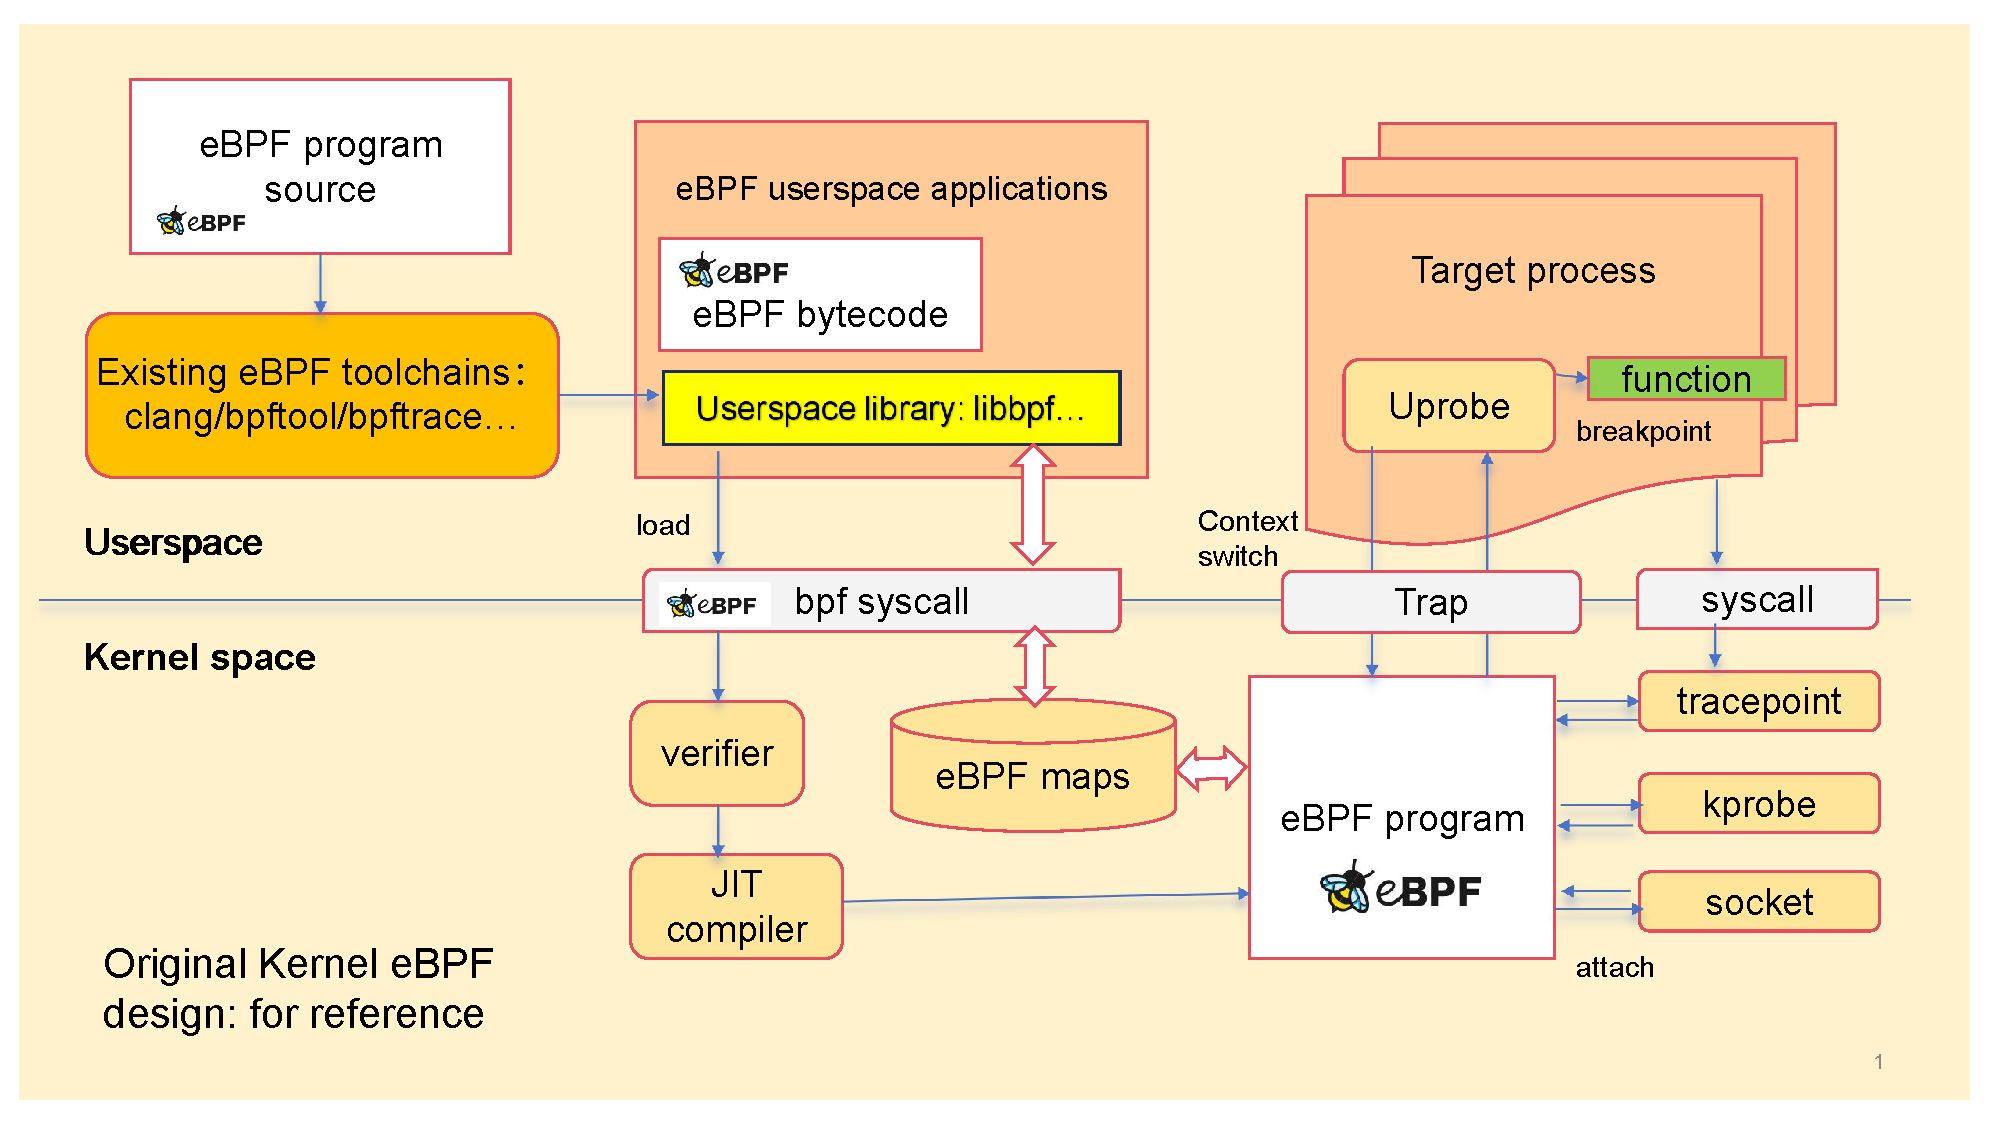
\includegraphics[width=0.5\textwidth]{img/bpftime1.pdf}
\caption{The Workflow of kernel eBPF runtime}\label{fig:workflow}
\end{figure}

\subsection{Uprobe and Syscall Tracepoints}

Uprobes and syscall tracepoints are fundamental mechanisms that enable interaction and introspection within the kernel, particularly when used alongside eBPF. 

\textbf{Uprobes}, which stand for user-level dynamic tracing \cite{keniston2007ptrace}, and are part of perf-tools, allow for dynamic instrumentation of any routine in the user space, facilitating the collection of crucial data for performance analysis and fault diagnosis. Unlike kprobes, which operate within the kernel, uprobes trap into the kernel using the int3 instruction and execute in the kernel space with kernel eBPF, incurring a significant overhead due to the two context switches required - one into the kernel and another back out to the user space. This overhead can often result in a 10 to 20 times slowdown, make it not suitable for real-time monitoring in latency-sensitive applications. Despite the overhead, the combination of uprobes and the eBPF framework provides a powerful tool for non-intrusive tracing of user space functions without necessitating recompilation or restarting user space processes. This has led to its wide adoption in production environments. For instance, uprobes have been utilized for SSL/TLS data capture \cite{ecapture}, memory allocation monitoring and goroutine tracing\cite{bcc} in notable open-source projects. Additionally, they play a significant role in Distributed Tracing Troubleshooting in Zero Code environments, aiding in the identification and resolution of system issues with minimal intrusion into running processes\cite{shen2023network}.

\textbf{Syscall tracepoints} provide a simple way to intercept and modify system calls throughout the system, becoming powerful tools for security and monitoring when used with eBPF. With eBPF, syscall tracepoints can be set up to react to or change system call parameters and return values, allowing detailed control and monitoring of system interactions. In action, when a system call is made, the relevant syscall tracepoint is triggered, starting the connected eBPF program. This eBPF program can inspect the system call parameters, make decisions based on its rules, and even change the return value of the system call. For instance, an eBPF program can be set to block certain system calls by changing the return value to an error code, offering a straightforward way for system call filtering crucial for security. Tracepoints were among the early features brought in with eBPF and have gained wide usage due to their reliability. Unlike kprobes, syscall tracepoints provide a more stable interface and can be used reliably across different kernel versions, making them a favored choice for many. The clear-cut interface of syscall tracepoints reduces the chance of inconsistencies across different kernel versions, establishing the pairing of syscall tracepoints and eBPF as a strong solution for system-wide interception and alteration of system calls.

\subsection{Userspace lightweight isolation: eBPF and Wasm}

The realm of userspace virtual machines has seen the advent of two notable runtimes: eBPF (Extended Berkeley Packet Filter) and Wasm (WebAssembly). Each of these runtimes has distinct design philosophies and operational principles, which cater to varying use-cases and operational requirements.

eBPF, originally rooted in the kernel space, migrated to userspace to alleviate some challenges associated with kernel-based execution. The migration was pioneered by projects like uBPF and rbpf, which aimed to harness the robust capabilities of eBPF while ensuring safer and more convenient user-space operations \cite{ubpf, rbpf}. However, these initial attempts encountered hurdles including the lack of comprehensive support for uprobes and syscalls, the need for manual compilation and program restarts for integration, and an underwhelming hashmap implementation. Despite these limitations, these projects showcased the potential of userspace eBPF runtimes and paved the way for further advancements. For instance, frameworks like RapidPatch and Femto-Containers leveraged eBPF for patch propagation and secure deployment on embedded and IoT devices, demonstrating the versatile applications of eBPF \cite{rapidpatch, femto}. Moreover, projects like DPDK and the ongoing eBPF for Windows initiative indicate substantial progress towards utilizing eBPF benefits across a broader spectrum of applications and platforms \cite{dpdk-ebpf, windows-ebpf}. eBPF prioritizes performance, employing a verifier to ensure security, albeit placing it as a secondary concern.

On the other hand, Wasm is a well-established userspace virtual machine, extensively adopted as a plugin system and a lightweight containerization solution. Its wide language support enables the execution of entire libraries or processes, fostering a rich ecosystem for development. However, Wasm presents some limitations, particularly when it comes to integration. Manual integration is often required, making it less adaptable to API version changes. It relies heavily on underlying libraries for complex operations, such as Wasi-nn, and external APIs like Wasi necessitate additional validation and runtime checks, leading to high performance costs. Unlike eBPF, Wasm emphasizes security, employing Software Fault Isolation (SFI) for security, even at the expense of some runtime overheads.

Both eBPF and Wasm exemplify the strides made in userspace virtual machine technologies, each with its unique strengths and challenges. Their comparative analysis provides a richer understanding of the landscape and the trade-offs involved in leveraging these runtimes for different application domains.
% \section{Related Work}\label{sec:related_work}
% go back
\sys is the first system to support comprehensive, safe, dynamic, and efficient extensions. 

Many systems support software customization through an extension primitive allowing developers to observe or modify a system's default behavior.  Nearly all existing work supports extending either an operating system kernel (\eg Nooks~\cite{Swift03}, VINO~\cite{Seltzer96}, SPIN~\cite{Bershad95}) or an application (\eg PIN~\cite{Luk05}, Valgrind~\cite{Nethercote07}, DynamoRIO~\cite{Bruening12}).  In contrast to these systems, \sys supports comprehensive extensions---\ie ones that extend both userspace applications and a kernel.

eBPF is the de facto extension framework in linux and has recently been adopted in Windows~\cite {eBPFWindows}.  eBPF is \emph{almost} comprehensive, except that eBPF userspace extensions cannot modify application behavior.  Moreover, eBPF's appraoch to safety executes userspace extensions in the kernel which comes with high overhead.  \sys{} resolves the comprehensiveness and efficiency issues of eBPF by executing userspace extensions directly in the execution context of the target application without requiring kernel involvement.

Ensuring system safety in the presence of software extensions requires isolating extension logic from the original logic of the program.  Many systems isolate untrusted extension code in a sandbox through the use of software fault isolation (SFI)~\cite{Wahbe93}.  For example,  dynamic instrumentation frameworks~\cite{Luk05, Nethercote07, Bruening12}, and lightweight virtual machines (\eg WebAssembly~\cite{webassembly}, NaCL~\cite{Yee09}, RLBox~\cite{Narayan20}), execute programs in a virtualized environment that monitors all memory and control-flow operations to isolate failures.  These approaches impose a high runtime overhead that precludes efficiency.

\sys{}'s use of intra-process memory protections is adopted from the approaches taken by Donky~\cite{schrammel2020donky}, ERIM~\cite{Vahldiek19} and libmpk~\cite{Park19}.  \sys{}'s key differences between these systems is the target domain---\sys{} applies these ideas to extend an existing application without requiring source-code changes, whereas prior work uses intra-process memory protection to provide lightweight protection domains that a rewritten application can use. There are many lightweight isolation abstractions that have been proposed (\eg Wedge~\cite{Bittau08}, Lightweight contexts~\cite{Litton16}, Orbit~\cite{Jing22}, \etc); \sys{} differs from these works in its target domain.

ubpf~\cite{ubpf} and rbpf~\cite{rbpf} implement virtual machines for executing eBPF bytecode in userspace.  These systems have higher runtime overhead compared to \sys's runtime that uses LLVM's ORC JIT\cite{Lattner04,lu2022bring} (see \cref{sec:design}).  Additionally, ubpf and rbpf are incomplete in that they do not support as many eBPF features as \sys and do not support eBPF Maps.

%\yusheng{
%The ubpf uses handwritten single pass jit, without doing much optimization. The rbpf is using cranelift JIT, and \sys is using LLVM jit. The \sys jit is faster thanks to the optimization from LLVM. We lift the bpf bytecode to llvm bytecode, and config llvm passes to optimize it.(Try to maximize the optimization level). The performance evaluation can be provided.

%Also, they doesn't support as many eBPF features as \sys. For example, they doesn't support atomic eBPF instructions.We have a conformance test for it, many we can put the compare in evaluation?

%This is for the eBPF virtual machine, but I think the most difference between the \sys and ubpf/rbpf is that they doesn't support eBPF maps in share memory or in kernel, and they cannot attach to userspace functions or syscalls, also they cannot dynamically inject in to a running process. They are just virtual machines.} \arq{thanks!}

\begin{comment}

\subsection{Dynamic Binary Instrumentation}

Dynamic Binary Instrumentation (DBI) facilitates real-time analysis of binary applications by injecting instrumentation code during runtime. This mechanism permits the embedding of specific analysis code into a program as it executes, tailored to user specifications, without disrupting the dynamic execution flow of the program. Renowned platforms that provide dynamic binary analysis capabilities include Pin\cite{1550984}, DynamoRIO\cite{dynamorio}, and Frida\cite{fridagum}. The defining attributes of DBI encompass its capability to work directly on binary code, obviating the need for source code, and its dynamic modus operandi which allows on-the-fly modifications to the program, thus negating the necessity for recompilation or program restarts. Nonetheless, DBI comes with certain caveats: it lacks built-in security checks or verification measures which may pose potential security risks. Moreover, in the absence of a high-performance virtual machine (VM) and an encapsulated sandbox environment, the efficiency of DBI could be compromised, and there's a potential to disrupt the execution states of the target process. Furthermore, existing DBI tools fall short in providing a high-performance control panel or data aggregation mechanisms akin to the capabilities offered by eBPF maps.

\subsection{WebAssembly}

WebAssembly (Wasm)\cite{webassembly} is a binary instruction format created as a portable compilation target for high-level languages such as C, C++, and Rust. It endeavors to achieve execution at native speed by leveraging common hardware capabilities. WebAssembly's design ensures portability across all modern platforms, both on desktop and mobile. It also operates within a sandboxed execution environment to maintain secure execution. With its binary format, WebAssembly enables faster parsing, compiling, and execution compared to traditional text-based web technologies. The structure and principles behind WebAssembly make it a suitable platform for various use cases beyond the web, including blockchain, serverless computing, and portable CLI tools, among others.

Both Dynamic Binary Instrumentation and WebAssembly illustrate unique approaches to runtime code analysis and execution. While DBI offers detailed insights into binary code behavior during runtime, WebAssembly provides a secure and portable compilation target. The exploration of these technologies, alongside the development of \textit{bpftime}, contributes to the broader effort of advancing runtime code analysis and execution frameworks.

\end{comment}
% \section{\sys Challenges}\label{sec:challenges}
\begin{figure}[t]
% \centering
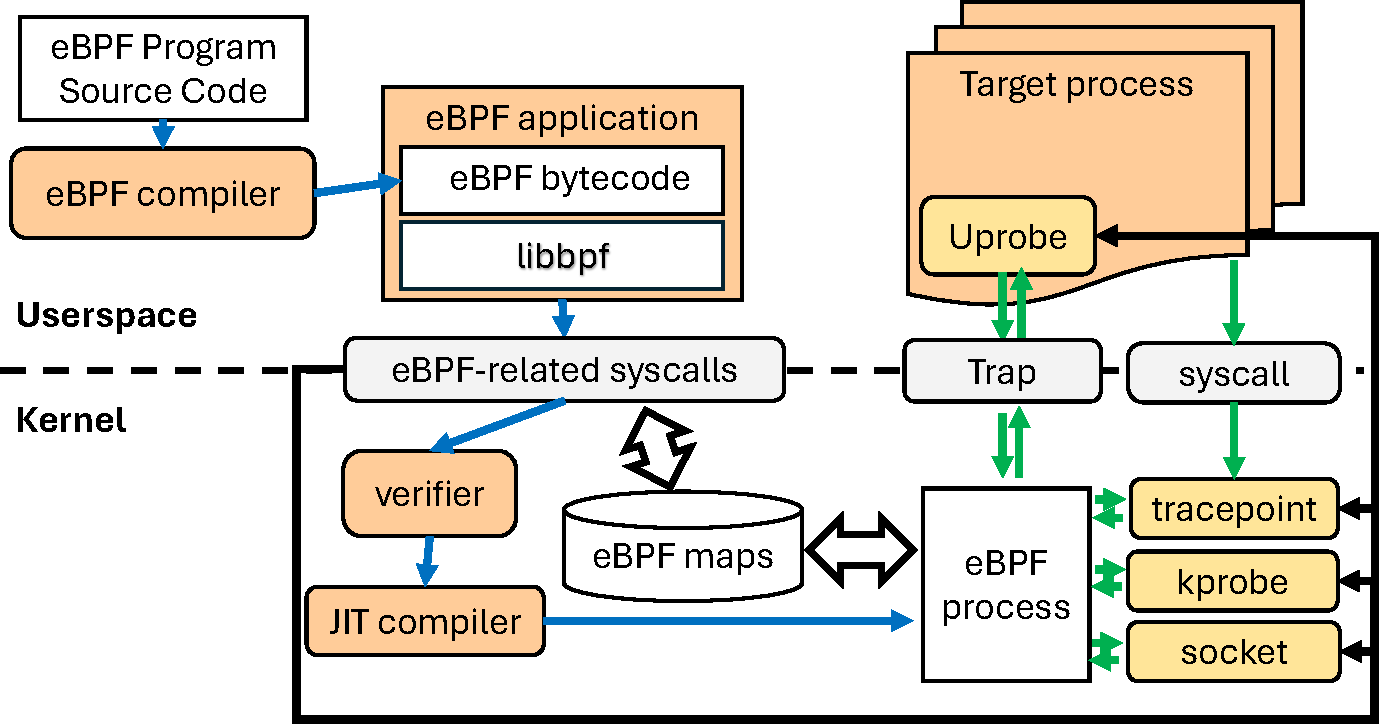
\includegraphics[width=\columnwidth]{img/ebpf-diagram-cropped.pdf}
\caption{eBPF Design Diagram.  Blue arrows indicate the execution flow when a user compiles and loads an eBPF program.  Green arrows indicate the execution flow when an eBPF extension executes.  White arrows with black outline indicate read/write operations to shared memory in the eBPF maps.  Black arrows indicate operations that attach an extension}\label{fig:eBPF-design}
\end{figure}

\sys{} is a comprehensive dynamic, safe, and efficient extension framework.  The system builds on the success of the eBPF ecosystem, which provides many of the design constraints.  However, \sys{} crucially diverges from eBPF in its technique to support extensions to userspace logic.  Namely, rather than execute userspace extension logic in the kernel, which degrades comprehensiveness and efficiency, \sys{} instead creates a new userspace eBPF runtime that uses dynamic binary instrumentation to execute userspace extensions directly in the extended application.

However, execute eBPF extensions in userspace leads to three main challenges: \sys{} must provide a new eBPF runtime, \sys{} must devise a new method for attaching to an arbitrary program, and \sys{} must ensure safety of the user's extensions. 

In the remainder of this section, we first provide background on the current eBPF ecosystem (\cref{sec:challenges:eBPF-background}).  Then, we outline the challenges that arises when extending eBPF execution into userspace (\cref{sec:challenges:details}). 

\subsection{eBPF Background} \label{sec:challenges:eBPF-background}
This section describes the background eBPF knowledge necessary to understand \sys{}.  \Cref{fig:eBPF-design} shows a design diagram of the critical components of the ecosystem and how the components interact.  We discuss the three main phases of interacting with eBPF: Writing an eBPF program, loading an eBPF program, and executing an eBPF program.

\subsubsection{Writing an eBPF program}

A user writes an eBPF program (eBPF Program Source Code).  The user expresses each of the extensions that they wish to add to the system as a separate function. They annotate the hook point for each extension using the syntax \mintinline{c}{SEC("<type>/<name>")} indicating that the function should be executed when the program reaches the hook point \mintinline{c}{name} of probe type \mintinline{c}{type} (\eg \texttt{kprobe}, \texttt{uprobe}, \texttt{uretprobe}, etc.).  The user can leverage a rich set of eBPF helper functions to help with many tasks, including access eBPF maps, read memory, get process information, etc.   The user passes their eBPF program to an eBPF compiler (e.g., \texttt{clang}), which produces eBPF bytecode for the user's extensions. The bytecode consists of the program's extension logic (\ie its functions), maps and their associated hook points as an ELF binary.  

\subsubsection{Loading an eBPF Program}

When the user wishes to execute their extension, they use an existing toolchain (e.g., \texttt{libbpf}) to load the eBPF bytecode.  The toolchain interacts with a number of bpf-related system calls (\eg \mintinline{c}{bpf}, \mintinline{c}{perf_event_open}) to load the extension into the system.  The bpf-related system calls perform three main tasks.  First, some of the eBPF system calls initialize maps for the eBPF program to use. Second, some of the eBPF system calls instrument the actual hook points (e.g., \texttt{uprobe}s, \texttt{kprobe}s, etc.) required by the eBPF program.  The instrumentation adds software breakpoints (\ie \texttt{int 0xcc}) for userspace hook point, and uses trampolines (\ie \texttt{jmp} instructions) for kernel space hook points.  Finally, some of the eBPF system calls validate the eBPF byte code. These calls pass the eBPF bytecode for the user's execution logic to an eBPF verifier.  One important note: the current eBPF ecosystem \emph{does not} verify userspace extensions (\ie those that attach to \texttt{uprobe} and \texttt{uretprobe} hook points).
\yusheng{Might be better to describe as "does not ensure userspace extensions don't break userspace process." because it does verify the uprobe eBPF don't break kernel, like infinity loop or access kernel memory wrong.} \arq{OK. I'm totally confused, then.  I thought that eBPF's uprobes are not able to change the state of the userspace program.  So, I don't understand the distinction that you're drawing here...}

The verifier uses static analysis to ensure that the eBPF bytecode is safe to execute.  Namely, the verifier checks to see if the eBPF bytecode is memory and type safe by checking the type and memory offset of each memory dereference in the bytecode by consulting metadata released with each kernel called the BPF Type Format (BTF).  Next, the verifier ensures that the bytecode terminates by ensuring that all loops have a constant bound, are not recursive.  The verifier validates that there are no hardware exceptions in the eBPF bytecode by checking each instruction.  For example, it checks for divisions by unknown scalars to ensure that an extension cannot cause a divide-by-zero exception.  Lastly, the bytecode verifier ensures that the extension does not leak resources by ensuring that all allocated resources (e.g., ring buffer memory) are released on all possible program paths.

\subsubsection{Executing an eBPF Program}

After the eBPF program is loaded, the system begins executing.  The kernel provides a Just-in-time (JIT) Compiler that takes the verified eBPF bytecode as input and compiles it as necessary to the native architecture of the machine.  The system executes the eBPF bytecode logic each time it reaches a configured hook point.  When the kernel reaches a kernel hook point, the trampoline technique redirects execution to the eBPF extension.  When the userspace application reaches a hook point, the application executes a trap which passes control to the eBPF extension.  This incurs at least two context switches (one to the kernel and one back to userspace), often even more as the system must execute the logic of the instruction located at the software breakpoint, which comes with high overhead.

The eBPF extensions read and modify the system's state.  They use eBPF maps to store execution state across extended hook points, and also to communicate output data to the eBPF application.  The eBPF application can use system calls to read this data, primarily in observability use-cases. 

\subsubsection{DeepFlow Example}
\begin{figure}[t]
\centering
\begin{minted}{c}
struct event {
  u32 saddr_v4;
  u64 goid;
};

BPF_RINGBUF_OUTPUT(rb, 1 << 4);
BPF_HASH(goroutines, u64);

SEC("uprobe/go-server-http:runtime.casgstatus")
int uprobe_runtime_casgstatus(struct pt_regs * ctx) {
  void *gp = ctx->ax;
  u64 goid;
  if (bpf_probe_read_user(&goid, sizeof(goid),
                          gp + GOID_OFFSET) == 0) {
    u64 thread = bpf_get_current_pid_tgid();
    bpf_map_update_elem(&goroutines, &thread, &goid, 0);
  }
  return 0;
}

SEC("kprobe/tcp_v4_connect")
int BPF_KPROBE(tcp_v4_connect, struct sock* sk) {
  u64 thread = bpf_get_current_pid_tgid();
  u64 *goid_p = bpf_map_lookup_elem(&goroutines, &thread);
  if (!goid_p)
    return 0;
  struct event* data;
  data = bpf_ringbuf_reserve(&rb, sizeof(*data), 0);
  if (!data)
    return 0;
  BPF_CORE_READ_INTO(&data.saddr_v4, sk,
    __sk_common.skc_rcv_saddr);
  data->goid = *goid_p;
  bpf_ringbuf_submit(data, 0);
}
\end{minted}
\vspace{-0.5cm}
\caption{A simplified eBPF implementation of DeepFlow. \arq{A few things: First, the definition of goroutoine\_execute\_data is not provided.  Second, I updated the output to be an actual use-cases that someone might do.}} \yusheng{I change it slightly, add data defines and put a read tcp address here to make it correct. This is what people do.} \label{code:example}
\vspace{-0.5cm}
\end{figure}
We outline a small portion of the extensions for DeepFlow (see \cref{sec:motivation:examples}); \cref{code:example} provides the example code.  The program tracks the initial values of low-level socket options (\eg the size of a receive buffer), which are useful for identifying poor performance of socket related operations.  The program attaches logic on the userspace code that schedules \texttt{go-routine}s (\mintinline{c}{runtime.casgstatus}) to track the \texttt{go-routine} \texttt{ID} corresponding to each thread in the program.  It identifies the size of the receive buffer (\texttt{sk\_recvbuf}) of each tcp socket when the socket connects to an endpoint (inside the kernel at function \mintinline{c}{tcp_v4_connect}).  It produces output to a ring buffer of that shows the \texttt{go-routine ID} and the \texttt{sk\_recvbuf} value; the user's eBPF application correlates this output data with request-level tracing to identify if poor request performance is correlated with initial \texttt{sk\_recvbuf} values (this code is not shown).


\subsection{Userspace eBPF Challenges} \label{sec:challenges:details}

\sys{} resolves the efficiency and comprehensively challenges of the current eBPF ecosystem by executing userspace extensions directly in the target process.   The approach is conceptually simple, but it exposes a number of critical challenges: 

% \yusheng{ubpf and rbpf exist}  This includes the kernel's JIT Compiler as well as the many eBPF helper functions that the runtime provides to simplify eBPF program development.  Running an eBPF extension from userspace requires a new userspace runtime and new userspace helpers to fill these gaps.  \yusheng{The actually challenge is that 1. Our goal is provided compatible with existing eBPF toolchains and libraries, but the current eBPF loading process is complex, requires a sets of different syscall, include bpf, perf event open, mmap, epoll, open, close... syscalls, it's typically requires thousands of syscall executions to load and control all the eBPF programs in a eBPF application like deepflow. So the loader is complex and requires 4000 lines. If we don't provide compatibility to the toolchains, then it's impossible to run the large eBPF application like deepflow or even smaller bcc tools like sslsniff.} \yusheng{Another challenge is about eBPF maps. currently the eBPF ecosystem already has userspace jit implement, but not userspace maps implementation, especially we want to have shared maps between userspace and kernel, and shared maps between different userspace. We need to implement a lot of data structures in shared memory. This is critical for the execution of eBPF programs. I have discussed that in ppt.}

\paragraph{A New eBPF runtime for the eBPF Ecosystem} eBPF applications use a vast ecosystem of tooling, including a set of eBPF-related system calls, helper functions, eBPF maps, and eBPF JIT compilers, which must evolve to execute in userspace.  To ensure comprehensiveness, \sys{} must be  compatible this current ecosystem.  This includes seamlessly supporting current eBPF-related systemcalls, providing similar eBPF helper functions for userspace extensions, providing comprehensive eBPF maps, and providing a JIT compiler for executing eBPF code in userspace.  Prior work on userspace eBPF, including ubpf~\cite{ubpf} and rbpf~\cite{rbpf}, support JIT compilers for executign eBPF bytecode in userspace, but do not handle any of the other core issues. 


\paragraph{Attaching to an arbitrary program} The current eBPF ecosystem's logic for attaching to a userpsace program is a simple implementation that replaces program bytes with software breakpoints.  However, attaching to an arbitrary userspace process is significantly more difficult, especially to support extensions on \texttt{syscall tracepoints}, which need to instrument \emph{every} \texttt{sysenter} instruction in the program.  Solving this challenge is paramount for ensuring that \sys{} is efficient.

\paragraph{Safety} Executing userspace extensions exposes the system to two safety problems.  First, the kernel's verifier assumes that eBPF bytecode executes over the kernel's runtime and ecosystem, so \sys cannot use it to ensure that a buggy extension cannot crash the system.  Second, executing the extension within the target process renders it susceptible to compromise by a subverted application.  Preventing such attacks requires that \sys{} ensure (1) that the target process cannot modify the extension logic and (2) that the memory used by the eBPF extension can be shared across userspace and kernel extensions without being read/written by the extended process.


\section{Approach and Challenges}\label{sec:challenges}
\begin{figure}[t]
% \centering
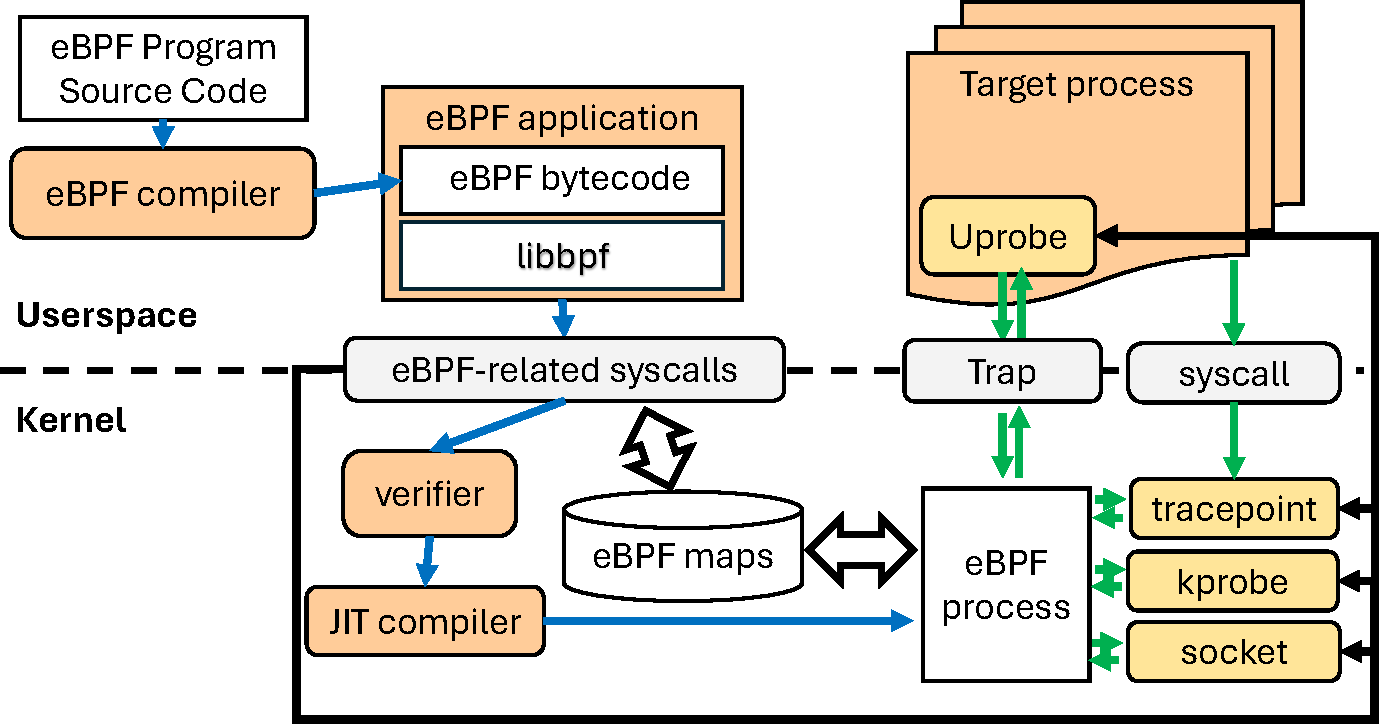
\includegraphics[width=\columnwidth]{img/ebpf-diagram-cropped.pdf}
\caption{eBPF Design.  Blue arrows show execution flow when compiling and loading an eBPF application. Green arrows show execution flow when an eBPF extension executes.  White arrows with black outline indicate components that interact with eBPF maps.}\label{fig:eBPF-design}
\end{figure}

Our goal is to build a comprehensive, dynamic, safe, and efficient extension framework.  Our approach centers around two guiding design principles.  First, we seek to leverage the success and industry clout of the existing eBPF ecosystem.  To this end, we will {\em maintain compatibility} with applications and extensions built for the current state of the art eBPF framework.  As described above, eBPF satisfies many of the design constraints, but degrades comprehensiveness and efficiency by executing userspace extension logic in the kernel.  To remedy this, as the second guiding principle, we seek to run user extensions entirely in userspace {\em without requiring kernel involvement}, even as they inter-operate with other eBPF extensions in the kernel or elsewhere in the system. %\arq{One downside of how these are presented is that they don't point back to the design goals established in the previous section} \yusheng{I think the four princeples, comprehensive, dynamic, safe, and efficient are for the general extension systems. Since we choose eBPF, we want our new extension system still supports a large ecosystem exists in the world, and can run complex, real world extension applications. So this is the main design constrains for our extension system besides the four lists before.} \yusheng{They are mainly for "keep comprehensive, dynamic, safe, and efficient, and also able to run real-world non-trival extension tasks in real world production systems"}

In the remainder of this section, we first provide further background
on the current eBPF ecosystem (\cref{sec:challenges:eBPF-background}).
Then, we outline the challenges that arises when extending eBPF
execution into userspace (\cref{sec:challenges:details}).


\subsection{eBPF Background} \label{sec:challenges:eBPF-background}

This section describes the current eBPF framework. \Cref{fig:eBPF-design} shows the  critical components of the ecosystem and how their interaction.  We discuss the three main phases of interacting with eBPF: writing an eBPF program, loading an eBPF program, and executing an eBPF program.


\subsubsection{Writing eBPF Applications}

An eBPF application consists of two components: (1) the code that will run in the context of the larger system to perform tracing or customization, called the {\em extension} or {\em eBPF program}; and (2) the userspace control plane application that loads one or more extensions and later communicates with them (e.g., to extract and/or analyze data), called the {\em eBPF application}.  

The user writes an eBPF program (eBPF Program Source Code), by specifying a set of functions that will execute in an event-based manner.  Each function will execute when the attached program reaches a configured event, called a \emph{hook point}, specified using a symbolic name (e.g., a function name in the kernel or a path to an executable and function name for user applications).  There are many possible hook points from general (\texttt{uprobe}s, \texttt{kprobe}s, etc.) to specific (XDP~\cite{vieira2020fast}, seccomp~\cite{seccomp-ebpf}, etc.).  The most general hook points are \texttt{uprobe}s and \texttt{kprobe}s, which support extending any userspace or kernel instruction, respectively.  eBPF programs can use a rich set of {\em eBPF helper functions} for reading memory, obtaining process information, etc.  Importantly, the eBPF framework provides helper APIs so that programs can store state in buffers called {\em maps} to communicate with other extensions, the control plane eBPF application, the external system, or a future invocations of the same eBPF extension.  Extensions are typically written in C, with hook points specified as section names that will be interpreted by the eBPF application at load time using a library such as libBPF.

The user passes their eBPF program to an eBPF compiler (e.g., \texttt{clang}), which produces an ELF binary containing the program's extension logic (\ie its functions) represented in eBPF bytecode, their associated hook points as an ELF binary, and information about the maps for the eBPF progrma. 

An eBPF application forms the control plane of a distributed set of extensions.  It is responsible for loading, communicating with and coordinating extensions, and, as such, can be very complex.  Due to the breadth and complexity of these applications, compatibility with the current eBPF ecosystem (our first guiding design principle) is critical.

%% A user writes an eBPF program (eBPF Program Source Code).  The user expresses each of the extensions that they wish to add to the system as a separate function. They annotate the hook point for each extension using the syntax \mintinline{c}{SEC("<type>/<name>")} indicating that the function should be executed when the program reaches the hook point \mintinline{c}{name} of probe type \mintinline{c}{type} (\eg \texttt{kprobe}, \texttt{uprobe}, \texttt{uretprobe}, etc.).  The user can leverage a rich set of eBPF helper functions to help with many tasks, including access eBPF maps, read memory, get process information, etc.  \Cref{code:example} provides a simple but realistic eBPF program that finds which go-routine is accepting TCP connection and report the event to userspace eBPF application. The uprobe program gets the relation between go-routine ID and thread ID, store it into the hash map. The kprobe program is triggered on tcp connect events, get the related go-routine ID from hash map and report the event to userspace with ring buffer.

%% The user passes their eBPF program to an eBPF compiler (e.g., \texttt{clang}), which produces eBPF bytecode for the user's extensions. The bytecode consists of the program's extension logic (\ie its functions), maps and their associated hook points as an ELF binary.  

\subsubsection{Loading and Attaching eBPF Programs}

Regardless of whether an eBPF program will extend the kernel or a userspace application, the eBPF application utilizes kernel system calls to create any required maps, load each eBPF program, and attach each program to the specified hook point.  This is typically accomplished via a library, such as libBPF.

When a user loads an eBPF program, the kernel ensures that the eBPF bytecode is safe to execute using static analysis.  Namely, the in-kernel verifier checks if the eBPF bytecode is memory and type safe by checking the type and memory offset of each memory dereference in the bytecode using metadata released with each kernel called the BPF Type Format (BTF).  Next, the verifier ensures that the bytecode terminates by ensuring that all loops have a constant bound and are not recursive. The verifier also validates that there are no hardware exceptions in the eBPF bytecode by checking each instruction.  For example, it checks for divisions by unknown scalars to ensure that an extension cannot cause a divide-by-zero exception.  Lastly, the bytecode verifier ensures that the extension does not leak resources by ensuring that all allocated resources (e.g., ring buffer memory) are released on all program paths.

%The purpose of the verifier is to protect the system (kernel or userspace process) from a misbehaving extension.  However, while it does protect against some common mistakes, the verification is not sufficient to protect from an extension that purposefully performs customization or misuses helpers~\cite{hotos-untenable}.  The verifier does not protect the extension from the system.  However, userspace extensions are protected from the application they are attached to by nature of running in kernel context (discussed next). \arq{While this is all true, I'm wondering if it is totally worth bringing up here, given that we don't have an answer to the concern.} \yusheng{I think maybe we can try to simplify some of the verifier part here?}

Once the verifier is satisfied with the extension bytecode, the kernel compiles it into native code with an in-kernel just-in-time (JIT) compiler.  When instructed to do so via a system call, the kernel attaches the compiled extension program to a hook point.
%There are many possible hook points that an extension can be attached to ranging from general (\texttt{uprobe}s, \texttt{kprobe}s, etc.) to specific (XDP~\cite{xdp}, seccomp~\cite{seccomp-ebpf}, etc.).  The most general hook points are \texttt{uprobe}s and \texttt{kprobe}s, which allow attachment to any userspace or kernel instruction, respectively.  
When attaching an eBPF program to these hook points, the kernel modifies user or kernel code by adding software breakpoints (\ie \texttt{int 0xcc}) that will trap when executed.\footnote{In the kernel, some {\texttt kprobe}s are
optimized to use non trapping instructions.}


%% When the user wishes to execute their extension, they use an existing toolchain (e.g., \texttt{libbpf}) to load the eBPF bytecode.  The toolchain interacts with a number of bpf-related system calls (\eg \mintinline{c}{bpf}, \mintinline{c}{perf_event_open}) to load the extension into the system.  The bpf-related system calls perform three main tasks.  First, some of the eBPF system calls initialize maps for the eBPF program to use. Second, some of the eBPF system calls instrument the actual hook points (e.g., \texttt{uprobe}s, \texttt{kprobe}s, etc.) required by the eBPF program.  The instrumentation adds software breakpoints (\ie \texttt{int 0xcc}) for userspace hook point, and uses trampolines (\ie \texttt{jmp} instructions) for kernel space hook points.  Finally, some of the eBPF system calls validate the eBPF byte code. These calls pass the eBPF bytecode for the user's execution logic to an eBPF verifier.  One important note: the current eBPF ecosystem \emph{does not} verify userspace extensions (\ie those that attach to \texttt{uprobe} and \texttt{uretprobe} hook points).
%% \yusheng{Might be better to describe as "does not ensure userspace extensions don't break userspace process." because it does verify the uprobe eBPF don't break kernel, like infinity loop or access kernel memory wrong.}

%% The verifier uses static analysis to ensure that the eBPF bytecode is safe to execute.  Namely, the verifier checks to see if the eBPF bytecode is memory and type safe by checking the type and memory offset of each memory dereference in the bytecode by consulting metadata released with each kernel called the BPF Type Format (BTF).  Next, the verifier ensures that the bytecode terminates by ensuring that all loops have a constant bound, are not recursive.  The verifier validates that there are no hardware exceptions in the eBPF bytecode by checking each instruction.  For example, it checks for divisions by unknown scalars to ensure that an extension cannot cause a divide-by-zero exception.  Lastly, the bytecode verifier ensures that the extension does not leak resources by ensuring that all allocated resources (e.g., ring buffer memory) are released on all possible program paths.

\subsubsection{Executing an eBPF Program}

After the eBPF program is loaded and attached, it will be invoked as the system executes.  Specifically, when the system encounters a trap, the kernel will execute the associated extension.   Note that the extension program runs in kernel context regardless of the hook point location. For userspace hook points, invoking the eBPF program incurs at least two context switches (one to the kernel and one back to userspace), and is often even more expensive as the system also must emulate the logic of the instruction replaced by the software breakpoint.  This significant overhead  prevents the existing eBPF framework from meeting the performance design constraint.

% As the eBPF program runs, it may utilize helper functions to read and modify the system's state and use eBPF maps to save system state across extension invocations, allowing extensions at different hook points and/or the eBPF application to cooperate to solve the user's problem. 

%% After the eBPF program is loaded, the system begins executing.  The kernel provides a Just-in-time (JIT) Compiler that takes the verified eBPF bytecode as input and compiles it as necessary to the native architecture of the machine.  The system executes the eBPF bytecode logic each time it reaches a configured hook point.  The eBPF bytecode read and modify the system's state and use eBPF maps to save system state across extension invocations, allowing extensions at different hook points to cooperate to solve the user's problem.  While the trampoline technique used for kernel hook points provides efficiency, the software breakpoint mechanism for \texttt{uprobe} or \texttt{uretprobe} does not.  Each userspace extension requires executing a trap.  This incurs at least two context switches (one to the kernel and one back to userspace), often even more as the system must execute the logic of the instruction located at the software breakpoint, which comes with high overhead.
%% L

\subsubsection{DeepFlow Example}
\begin{figure}[t]
\centering
\begin{minted}{c}
BPF_RINGBUF_OUTPUT(rb, 1 << 4);
BPF_HASH(goroutines, u64);

SEC("uprobe/go-server-http:runtime.casgstatus")
int uprobe_runtime_casgstatus(struct pt_regs * ctx) {
  void *gp = ctx->ax;
  u64 goid;
  if (bpf_probe_read_user(&goid, sizeof(goid),
                          gp + GOID_OFFSET) == 0) {
    u64 thread = bpf_get_current_pid_tgid();
    bpf_map_update_elem(&goroutines, &thread, 
                        &goid, 0);
  }
  return 0;
}

SEC("kprobe/tcp_v4_connect")
int BPF_KPROBE(tcp_v4_connect, struct sock* sk) {
  u64 thread = bpf_get_current_pid_tgid();
  u64 *goid_p = bpf_map_lookup_elem(&goroutines, 
                                    &thread);
  u64 data[2];
  data = bpf_ringbuf_reserve(&rb, sizeof(*data), 0);
  if (goid_p && data) {
      BPF_CORE_READ_INTO(&data[0], sk, 
                         __sk_common.sk_rcvbuf);
      data[1] = *goid_p;
      bpf_ringbuf_submit(data, 0);
  }
  return 0;
}
\end{minted}
\vspace{-0.5cm}
\caption{A simplified eBPF implementation of DeepFlow. 
\label{code:example}}
\vspace{-0.5cm}
\end{figure}
We describe a subset of the extensions for DeepFlow (see \cref{sec:motivation:examples}); \cref{code:example} provides the example code.  The program tracks the initial value of a socket option, the size of the receive buffer, to see if it is related to poor socket performance.  The program attaches logic on the userspace code that schedules \texttt{go-routine}s (\mintinline{c}{runtime.casgstatus}) to track the \texttt{go-routine} \texttt{ID} corresponding to each kernel thread.  It identifies the size of the receive buffer (\texttt{sk\_rcvbuf}) of each tcp socket at connection time (\mintinline{c}{tcp_v4_connect}).  It  outputs the \texttt{go-routine ID} and the \texttt{sk\_rcvbuf} value to aring buffer; the eBPF application correlates this output with request-level tracing to identify if poor request performance is correlated with initial \texttt{sk\_rcvbuf} values (this code is not shown).


\subsection{Userspace eBPF Challenges} \label{sec:challenges:details}

Our approach resolves the efficiency and comprehensively limitations of eBPF by executing userspace extensions directly in the target process without requiring kernel involvement.  Moreover, our approach maintains compatibility with applications and extensions built for eBPF.  This approach exposes three challenges: 

\paragraph{A New eBPF runtime for the eBPF Ecosystem} eBPF applications use a vast ecosystem of tooling, including a set of eBPF-related system calls, helper functions, eBPF maps, and a eBPF JIT compiler, which must evolve to execute in userspace.  Our approach must be compatible with this current ecosystem to ensure comprehensiveness.  This includes supporting eBPF-related system calls, providing similar eBPF helper functions for userspace extensions, providing comprehensive eBPF maps, and providing a JIT compiler for executing eBPF code in userspace.  Prior works on userspace eBPF (ubpf~\cite{ubpf} and rbpf~\cite{rbpf}) support userspace eBPF JIT compilers, but do not handle the other issues. 

\paragraph{Trap-free Userspace Extensions} Injecting a userspace extension in eBPF is simple: replace program bytes with software breakpoints (\ie traps).  However, traps require kernel involvement, violating the goal of kernel-free userspace extension execution.  Trap-free extensions in an arbitrary userspace process is difficult, especially to support extensions on \texttt{syscall tracepoints}, which must instrument \emph{every} \texttt{sysenter} instruction in the program.  

\paragraph{Safety} Executing userspace extensions exposes the system to two safety problems.  First, the kernel's verifier assumes that eBPF bytecode executes over the kernel's runtime and ecosystem, it cannot be used to ensure that a buggy extension cannot crash the system.  Second, executing the extension within the target process renders it susceptible to compromise by a subverted application.  Preventing such attacks requires (1) that the target process cannot modify the extension logic and (2) that the memory used by the eBPF extension can be shared across userspace and kernel extensions without being read/written by the target process.


%% \sys{} resolves the efficiency and comprehensively challenges of the current eBPF ecosystem by executing userspace extensions directly in the target process.   The approach is conceptually simple, but it exposes a number of critical challenges: 

%% \paragraph{A New eBPF Runtime and Ecosystem} The existing eBPF runtime can only be executed within the kernel; it does not work in a userspace context. \yusheng{ubpf and rbpf exist}  This includes the kernel's JIT Compiler as well as the many eBPF helper functions that the runtime provides to simplify eBPF program development.  Running an eBPF extension from userspace requires a new userspace runtime and new userspace helpers to fill these gaps. \yusheng{I think you might remove this paragraph because it's not challenge}
%% \yusheng{I think we have discussed this before? The challenge here is not the eBPF runtime itself, because there already exist 2 userspace jit eBPF runtime, ubpf and rbpf. it's also easy to implement the helpers.}
%% \yusheng{The actually challenge is that 1. Our goal is provided compatible with existing eBPF toolchains and libraries, but the current eBPF loading process is complex, requires a sets of different syscall, include bpf, perf event open, mmap, epoll, open, close... syscalls, it's typically requires thousands of syscall executions to load and control all the eBPF programs in a eBPF application like deepflow. So the loader is complex and requires 4000 lines. If we don't provide compatibility to the toolchains, then it's impossible to run the large eBPF application like deepflow or even smaller bcc tools like sslsniff.}
%% \yusheng{Another challenge is about eBPF maps. currently the eBPF ecosystem already has userspace jit implement, but not userspace maps implementation, especially we want to have shared maps between userspace and kernel, and shared maps between different userspace. We need to implement a lot of data structures in shared memory. This is critical for the execution of eBPF programs. I have discussed that in ppt.}
%% \yusheng{The attach complexity and safety complexity is exist.}

%% \yusheng{Suggested:}
%% \paragraph{A New eBPF Runtime for current Ecosystem} The existing eBPF applications like deepflow and bcc tools need a set of system call and hundreds to thousands of interactions with kernel to load their eBPF programs and maps. We need to provide compatibility with current bpf related syscalls to reuse the existing eBPF ecosystem and toolchains. There are already JIT compilers like ubpf and rbpf, but running eBPF programs in userspace still requires new eBPF maps implementation provide comprehensive, which is shared between kernel and userspace or different userspace processes to fill these gaps.

%% \paragraph{Attaching to an arbitrary program} The current eBPF ecosystem's logic for attaching to a userpsace program is a simple implementation that replaces program bytes with software breakpoints.  However, attaching to an arbitrary userspace process is significantly more difficult, especially to support extensions on \texttt{syscall tracepoints}, which need to instrument \emph{every} \texttt{sysenter} instruction in the program. 

%% \paragraph{Safety} Executing userspace extensions exposes the system to two safety problems.  First, the kernel's verifier assumes that eBPF bytecode executes over the kernel's runtime and ecosystem, so \sys cannot use it to ensure that a buggy extension cannot crash the system.  Second, executing the extension within the target process renders it susceptible to compromise by a subverted application.  Preventing such attacks requires that \sys{} ensure (1) that the target process cannot modify the extension logic and (2) that the memory used by the eBPF extension can be shared across userspace and kernel extensions without being read/written by the extended process.


\section{\sys Design}\label{sec:design}
\begin{figure*}[t]
% \centering
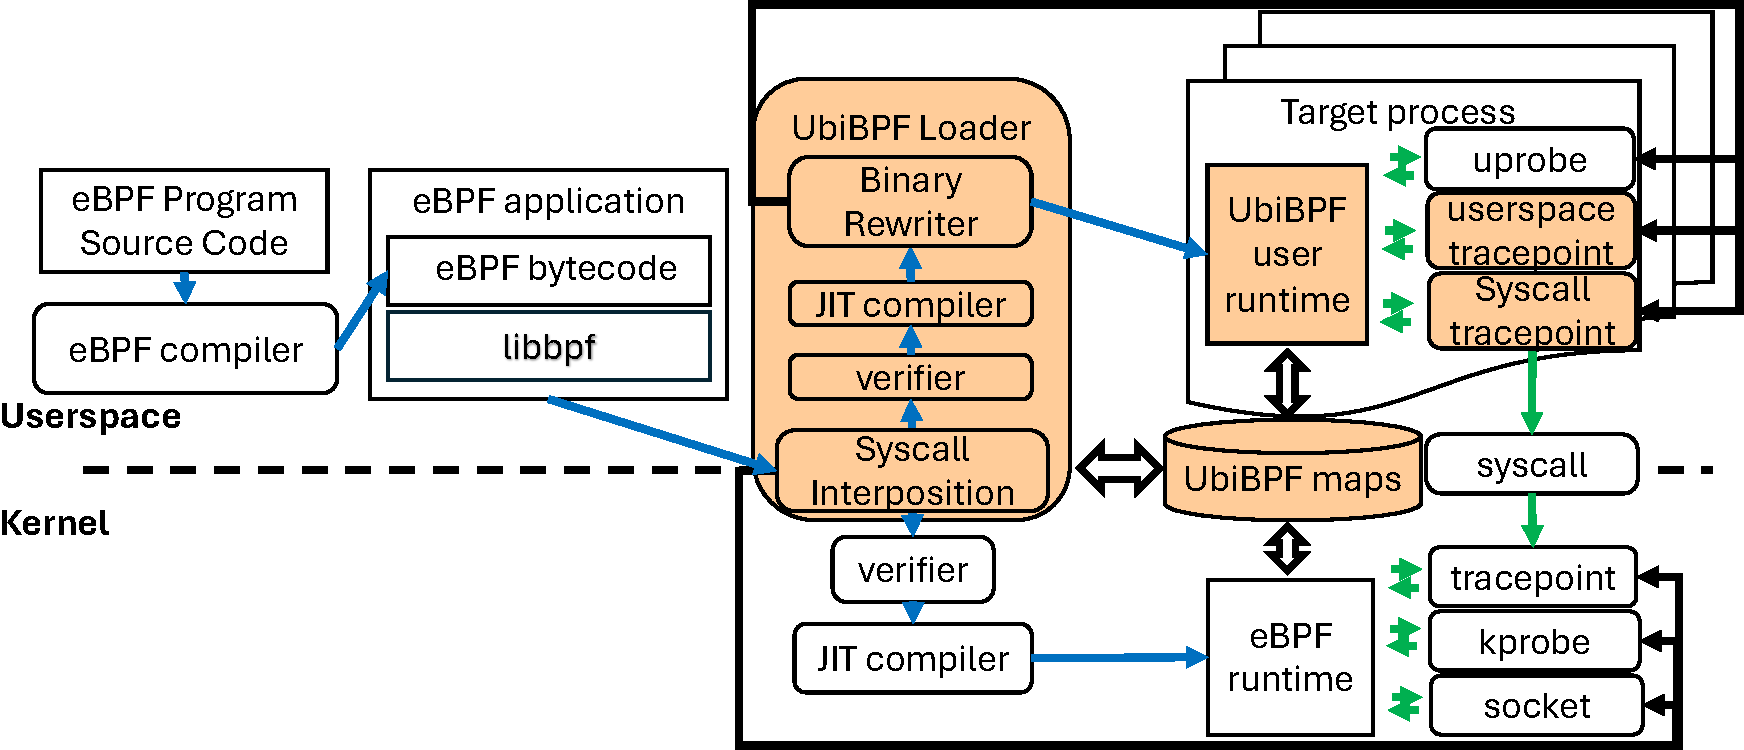
\includegraphics[width=.6\textwidth]{img/bpftime-diagram-cropped.pdf}
\caption{\sys{} Design.  White components are the same between \sys{} and eBPF; orange components are new to \sys{}. Arrow colors are consistent with \cref{fig:eBPF-design}. }\label{fig:bpftime-design}
\end{figure*}

\sys{} is a comprehensive, dynamic, safe, and efficient extension framework built using our two guiding principles: compatibility with the eBPF ecosystem and userspace extension execution without kernel involvement.  The system solves the three main challenges (\cref{sec:challenges}) that arise when following these principles: \sys{} solves the challenge of providing an eBPF-compatible runtime through the \sys{} Loader, a layer of interposition between the eBPF application and kernel that is feature-compliant with ebpf; the \sys{} maps, a new implementation of eBPF maps that allows userspace extensions and eBPF applications to interact without kernel involvement; and a collection of userspace eBPF helper functions.  \sys{} solves the challenge of trap-free extensions by adopting techniques from binary rewriting~\cite{Dinesh20, Chamith17, WilliamsKing20, fridagum}.  Finally, \sys{} ensures safety by using a userspace eBPF bytecode verifier~\cite{Gershuni19} to prevent a buggy extension from harming an application, and uses hardware memory protection~\cite{Vahldiek19, xie2022cetis} to prevent a buggy or subverted applications from circumventing an extension.  \Cref{fig:bpftime-design} shows the design.

\paragraph{Usage} \sys{}'s usage mirrors that of eBPF: a user writes an event-based eBPF program.  \sys{} provides a new type of hook point for the user, a \texttt{userspace} \texttt{tracepoint}, which an application developer can add to their code to support custom hook points, similar to \texttt{tracepoint}s in the kernel.  The user then compiles their program using an eBPF compiler.  At runtime, the user executes their eBPF application.  The eBPF application uses eBPF-related system calls, which the \sys{} loader interposes upon.  The loader verifies that the extensions are safe to execute, initializes data in the \sys{} maps for the application, initializes the \sys{} user and eBPF runtimes, and attach extensions to their hook points.  The \sys{} user runtime uses hardware isolation to ensure that extensions are safe from subverted applications.  During execution, the \sys{} user and eBPF runtimes execute extensions each time the userspace and kernel reach hook points, respectively.

The rest of this section describes \sys{}'s key components: the \sys{} loader (\cref{sec:design:loader}), the \sys{} user runtime (\cref{sec:design:UVM}), and the \sys{} maps (\cref{sec:design:maps}). 

\subsection{\sys Loader}\label{sec:design:loader}
The \sys{} loader prepares eBPF extensions in an eBPF application for execution.  The loader is a layer of interposition between an eBPF application and the kernel; it exposes the  eBPF-related system calls interface from the eBPF ecosystem, allowing \sys{} to support existing eBPF application frameworks (e.g., bcc and libbpf). 

The \sys{} loader first separates an eBPF application's extensions into userspace extensions and kernel extensions.  The system uses the conventional eBPF ecosystem's design to load kernel extensions; see \cref{sec:challenges:eBPF-background} for details. 

To load userspace extensions, the system first ensures that they are safe using an eBPF userspace verifier~\cite{Gershuni19}.  Similar to the in-kernel verifier (\cref{sec:challenges:eBPF-background}), the userspace verifier ensures that an extension is memory and type safe, guaranteed to terminate, and will not execute a hardware exception.  \sys{} adds two things to support its userspace eBPF bytecode verification.  First, it provides verification support for its userspace helper functions, including for map access (\cref{sec:design:UVM}).  Second, \sys{} parses DWARF debugging information to produce BTF information for the target application.  Once verified, extensions pass through a userspace JIT compiler, which compiles them into native code. The JIT compiler passes the compiled extensions to a binary rewriter. 

The binary rewriter uses \texttt{ptrace} to pause the target application and load the \sys{} user runtime (\cref{sec:design:UVM}) into it; this approach ensures dynamism.   The rewriter instruments the program's instructions to ensure that eBPF functions are invoked when the program reaches their associated \texttt{uprobe}, \texttt{uretprobe}, \texttt{syscall} \texttt{tracepoint}, or \texttt{userspace} \texttt{tracepoint}.  The rewriter supports \texttt{uprobe}s, \texttt{uretprobe}s, and \texttt{userspace tracepoint}s using a standard instruction trampoline: it replaces the instructions that were originally at the hook point with a \texttt{call} into a preamble for the point's associated eBPF function and places the overwritten instructions at the end of its preamble.  Supporting extensions to \texttt{syscall tracepoint}s is more complex.  Whereas other extensions should be invoked when a program reaches a specific userspace instruction, a extension to a \texttt{syscall tracepoint} should be invoked anytime the application executes a system call instruction (\ie \texttt{sysenter}), which are scattered throughout an application and its shared libraries.  To support this, the runtime iterates through all of the instructions in the application and places a trampoline on all system call instructions.  Since \texttt{sysenter} is smaller than a trampoline, the system uses zpoline~\cite{yasukata2023zpoline}, which uses the zero page to accommodate two-byte call instructions.

In addition to loading the eBPF extensions into the target application, the \sys{} loader also initializes the \sys{} maps required for the eBPF application. This process requires handling symbol relocations so that \sys{} can support multiple simultaneous eBPF applications.

% The \sys{} Daemon's eBPF bytecode verifier iterates through the instructions of the user-provided eBPF bytecode.  It ensures memory safety by checking that the type and memory offset of each memory dereference is correct by using the BPF Type Format (BTF).  The BTF includes low-level information about all structs referenced in the program, \eg their field offsets.  The verifier ensures termination by ensuring that all loops have a constant bound, are not recursive.% , and are not re-entrent (\ie they do not call any functions that they hook).   The verifier validates that there are no hardware exceptions in the eBPF bytecode by checking each instruction.  For example, it checks for divisions by unknown scalars to ensure that an extension cannot cause a divide-by-zero exception.  Lastly, the bytecode verifier ensures that the extension does not leak resources by ensuring that all allocated resources (e.g., memory) are released on all possible program paths.
%\yusheng{No re-enter is not guaranteed by verification, it's by runtime}\arq{does the kernel eBPF runtime ensure that there is no reentry as well?} \yusheng{Yes. guaranteed by runtime, there is some variables tracing this.}



\subsection{\sys User Runtime}\label{sec:design:UVM}
The \sys User Runtime executes userspace extensions.  Critically, the \sys{} user runtime provides safety. It ensures that a subverted application cannot affect or disable extensions through an intra-process memory isolation technology~\cite{Vahldiek19, xie2022cetis}.  \sys's approach differs from the isolation techniques used in existing extension frameworks (e.g. software-fault isolation) in that it occurs at load time and is thus less expensive.


\subsubsection{Safety mechanisms}

The \sys{} runtime uses memory protections, including page protections and intra-process memory protections (\eg Intel MPK), to ensure that extensions are safe from a subverted application.  The runtime ensures that the application cannot modify extension logic by setting the memory pages that contain an extensions and extension trampolines to be non-writable.  The runtime ensures the integrity of extension memory using intra-process memory protections~\cite{Vahldiek19, xie2022cetis}.  The \sys{} loader allocates a memory protection key for the extension's memory when it is loaded.  It adds instructions that use the allocated key (\ie \texttt{WRPKRU}) immediately before all userspace extensions, and adds instructions to reset the key immediately before returning to the original application.  To protect the key itself, \sys{} loads the key's value directly into the extension and sets the extension's memory permissions to be non-readable.

\subsubsection{Execution}

During execution, the \sys runtime is responsible for executing the eBPF bytecode of userspace extensions.  The execution occurs entirely in the original application, which ensures efficiency.   The runtime also includes a collection of helper functions to simplify extension development (\eg  \texttt{bpf\_override\_return}, a new helper that modifies the return value of a uprobe), and an interface called Userspace funcs (uFuncs), which allow an extension to execute functions from their host application or other libraries (\eg libc).  uFuncs are similar to the kfunc interface in eBPF.

\subsection{\sys Maps}\label{sec:design:maps}

\sys{} maps are a core component in ensuring comprehensiveness.   Conventional eBPF maps support userspace access through system calls. However, these system calls are expensive. So, \sys{} maps allow the \sys{} user runtime to allocate a shared memory region backed by \sys{} maps, following \sys{}'s design principle of userspace extension execution without kernel involvement. %\yusheng{This sentence seems a little hard to understand for me, maybe suggested:  So, \sys{} maps are designed so that the \sys{} user runtime can create shared memory for \sys{} maps between the application's address space and kernel, following \sys{} design principle of ensuring that userspace extensions execute without syscalls.} 
To ensure support verification of extensions that use \sys{} maps, the \sys{} maps include type information and behavior models describing the arguments and return values from \sys{} map helper functions. The \sys{} maps userspce helpers are highly efficient: they offer per-cpu variants to remove contention and use lock-free synchronization when necessary.
%\yusheng{Suggested add: The \sys{} Maps also provides necessary type info and behavior model for the eBPF verifier to ensure it's safe to shared between different runtimes.}

A user's eBPF application uses \sys{} maps to configure and consume the output of eBPF extensions.  eBPF supports these operations through eBPF-related system calls. \sys{} maintains compatibility with the existing eBPF ecosystem by interposing on the required system calls in the \sys{} loader and adding logic that uses \sys{} maps instead of the original eBPF maps. 

%Second, the userspace eBPF application access the maps with various syscalls(eg. bpf) and memory maps(eg. ring buffer). Since we have our own map implements, want to keep compatibility in order to run real world eBPF applications and don't want to modify the kernel, we need to mock the syscall and memory map operations for accessing and managing our own map implementation from the controller eBPF application.

%All the maps needs to be accessed are controlled by userspace eBPF application, like put config data in hash maps or receiving message from both eBPF runtimes, we provide additional mechanism for accessing and manage the userspace maps we managed in the \sys{} loader.


% First, most of the original eBPF maps are in the kernel context, they can only be accessed through syscalls, which are too expensive too used in user runtime. Array maps and ring buffer can be mmaped between kernel and userspace, but they are mainly designed for sending data from kernel to userspace, and don't meet our requirements for different kinds of maps, including hash maps, per-cpu maps, the ring buffer from user runtime to the controller application. We don't want to modify the kernel to support these features. Thus, we need to allow user runtime to have our own map implements in shared memory and manage them.


% designs
% In order to address these challenges, We first identify the maps need to be accessed by programs in userspace eBPF runtime. we will call these "userspace eBPF maps”, since they are managed and allocated by \sys{} user eBPF runtime. For the maps only accessed by kernel eBPF programs, they will remain untouched and manage by the kernel, so-called "kernel eBPF maps”. \arq{this does not really describe any design...?}

% If the maps also need to be shared with kernel eBPF runtime, we will create and manage the maps in a kernel array maps mmaped between kernel and userspace, and manage the actual map data struct in the shared buffer. 


% \yusheng{Note that access maps from the helpers in the runtimes and access from syscalls are different. For example, per cpu map has a copy on each cpu in the system to avoid locks. loopup elements in per cpu map from the helper side will only get the element from the map only for this cpu, but loopup elements from the syscall side will get the element from all the maps in all cpus. submit ring buffer and read ring buffer are also different because ring buffers are single direction. In helper side, performance is important, but in controller eBPF application, maps can be accessed by syscalls. We need to have different mechanism for them, both of them are reuired.}


% 1.We said that eBPF programs need to submit events to eBPF applications with ring buffer. But, the kernel only provides a single direction ring buffer, for example, kernel is the writer and userspace is the reader, you can submit the events from kernel to userspace, but you cannot submit events from a userspace eBPF runtime(process) to another userspace eBPF application (like deepflow)

% 2.there are "kernel maps" and "userspace maps". For example, the shared memory section we use to enable shared eBPF maps between kernel eBPF runtime and userspace eBPF runtime is managed by userspace bpftime. The kernel doesn't know what kinds of map it is, what's the type and which userspace eBPF program is using it, if we don't do any change in the eBPF application side, the application cannot access the maps we provided based on the original kernel mechanisms.

%The \sys{} Daemon allocates a new shared memory region for the extension to use, thereby ensuring that each extension has separate and isolated memory accesses.  The Daemon splits the allocation into distinct sections for program metadata (\eg hook locations, program names, etc), which it makes read-only, and memory for the extension to use as eBPF maps, which it makes read-and-write.  The Daemon exposes the allocated eBPF maps memory through the eBPF file system~\cite{bpffs}. \yusheng{The Daemon does not exposes the allocated shared memory through the eBPF file system~\cite{bpffs}. They are two completely different things. The bpffs is for eBPF maps shared  between userspace and kernel space, interact with kernel eBPF. The eBPF maps mmap between kernel and userspace and the shared memory we used are different. Maybe you can make it more clear here?}




%%% OLD GATE TEXT
%Third, when configured, \tech ensures that an extension protects all access to a \emph{region} of a program instructions by ensuring that all control flow from the application made to the region passes through the extension first. \sys employs hardware-supported control-flow integrity~\cite{cet} for this task; our prototype is built using Intel's indirect Branch Tracking (IBT)~\cite{gaidis2023fineibt,cet-ibt}.

%\subsection{Control-Flow Protection}\label{sec:tech:flow} When configured, \tech uses Control Flow Integrity, specifically Intel's IBT, to enforce that an application must execute an extension before executing the instructions in a region of memory (specified as a start instruction and a length).  The protection ensures that the malicious application can only execute instructions from the specified region by landing directly on the start instruction.  In essence, this control-flow protection ensures that a malicious application cannot bypass any monitoring or security enforcement that a \sys extension performs. 

% \tech uses static analysis and instruction rewriting together with IBT to enforce control-flow protection.  In brief, IBT issues a segmentation fault for any indirect branch whose target does not resolve to a special \texttt{ENDBR} instruction.  \tech rewrites the protected region to remove all such \texttt{ENDBR} instructions from the protected region, thereby preventing indirect control flow from reaching the region.  It issues a warning to the user if it identifies multiple such \texttt{ENDBR} instructions, as this is indicative of a incorrectly configured extension.  To protect against direct control-flow operations, \sys statically analyzes the application and issues an error if any control-flow operations land at a location inside of the protected region. 


\section{\sys Implementation}\label{sec:implementation}
We built a prototype of \sys{} in ~20,000 lines of C/C++ and ~1000 lines of python code.  One notable feature of the prototype is that \sys's kernel components are implemented entirely using the existing eBPF ecosystem, so the prototype \emph{does not} require any kernel modifications.  

The prototype consists of three main components: the \sys{} Loader (\cref{sec:design:loader}); the \sys{} User Runtime (\cref{sec:design:UVM}); and \sys{} Maps (\cref{sec:design:maps}).  Outside these components, the prototype includes ~3,000 lines of code for miscellaneous scripts (disassembly, examples, etc.).  We outline the core components of the prototype below.

\paragraph{\sys{} Loader}
The \sys{} Loader prototype consists of ~5,000 lines of code.  Most of this code (~3,000 lines) mocks system calls, which is required to load extensions, attach to userspace events, and manage \sys{} maps.  The prototype loader has two implementations: one includes a kernel component, implemented in eBPF, while the other is a userspace shared library that uses \texttt{LD\_PRELOAD} to mock system calls in libc.  The \sys{} loader prototype supports two eBPF bytecode verifiers for userspace extensions.  The system can use the in-kernel verifier, which offers support of all eBPF bytecode instructions but cannot verify extensions that use \sys{}'s custom helper functions, or PREVAIL, which supports all of \sys's custom helper functions but does not support all eBPF bytecode instructions.  Lastly, ~2000 lines of code in the loader are used to interact with \sys{} maps.



% One key challenge is producing the BPF Type Format (BTF) necessary for the verifier to ensure safety.  The Linux kernel maintainers produce the kernel's BTF alongside each release.  However, to verify an extension over an arbitrary userspace program, \sys must first produce the BTF for that program.  \sys produces BTF by first extracting debug information from the application, and then converting the debug information into BTF format.  If a function does not include debug information, then the verifier will restrict any eBPF functions from accessing the application's memory.  It also supports relocation in libbpf, allowing it to support the Compile Once---Run Everywhere (CO-RE) eBPF workflow.

%\yusheng{Maybe we can also mentioned compile once run everywhere here? It's a important feature of eBPF and we support it with userspace BTF}
% \yusheng{The Compile Once---Run Everywhere are supported in libbpf, which is part of the loading process and don't related to runtime. It's a different thing than uprobe attach to which functions, it's about whether the eBPF program works correctly even if the parameters/data structs changes}

\paragraph{\sys{} User Runtime}

The prototype user runtime consists of ~9,000 lines of code.  Roughly 3,000 lines of code are implement attaching logic, which uses Frida~\cite{fridagum} and libcapstone~\cite{libcapstone}.  \sys{} implements a new bytecode execution engine (~6,000 lines), since existing userspace eBPF engines (\eg uBPF~\cite{ubpf} and rBPF~\cite{rbpf}) impose high overhead and provide limited eBPF feature support.  The prototype execution engine uses LLVM's ORC Just-In-Time (JIT) Compiler~\cite{Lattner04, lu2022bring}.  At load time, the prototype compiles the eBPF bytecode into LLVM (IR); its execution engine converts the IR into native code during execution.  The prototype also supports an AOT compiler for resource limited devices.  The bytecode execution engine also includes the implementations of \sys{}'s helper functions and uFuncs interface.

\paragraph{\sys Maps}

The \sys{} Maps prototype (~4,000 lines) includes a rich set of map types and data structures, including hash maps, array maps, lpm tries, per-cpu hash and array maps, ring buffers and perf events arrays.  \sys{} allows eBPF applications and both runtimes (\ie the kernel and \sys{} user runtime) to use any of these data structures.  The \sys{} maps ensure efficiency by eliding system calls and use lock-free synchronization.  The prototype uses the eBPF file system~\cite{bpffs} to expose maps to the kernel and userspace.   This design ensures that accessing a \sys map does not require superuser privileges.


\input{tex/technique}
\section{Use Cases}\label{sec:use_cases}
We show the usefulness of \sys extensions across \numcases use cases that explore design tradeoffs, improve security, monitor performance, and improve performance.

\paragraph{DeepFlow}
DeepFlow uses all four of \sys{}'s constraints: comprehensiveness, dynamism, safety, and efficiency (see \cref{sec:motivation:examples}).  DeepFlow was originally implemented using the eBPF ecosystem, but eBPF \texttt{uprobe}s can result in as much as 50\% decrease in throughput.  We ported DeepFlow to \sys, modifying 10 out of the ~5,000 lines of eBPF code, so that the tool could benefit from \sys's efficiency.

\paragraph{Redis Durability Tuning}
%\begin{figure}[t]
%\centering
%\begin{minted}{c++}
%int writeback_fin_cnt; 
%// shared between kernel and userspace

%SEC("uprobe/fdatasync")
%int BPF_UPROBE(start_fsync, int __fd) {
%  if (writeback_fin_cnt == 0) {
%    io_uring_wait_and_seen();
%  } // else the fsync is completed 
%    // so we don't need to wait for CQE
%  successful_writeback_count = 0;
%  io_uring_prep_fsync(__fd);
%  io_uring_submit();
%  bpf_override_return(0, 0);
%  return 0;
%}

%SEC("kretprobe/file_write_and_wait_range")
%int BPF_KPROBE(file_write_and_wait_range, 
%              struct file *file, loff_t start,
%              loff_t end) {
%  ... // Check whether the fsync is 
%      // submited by the redis and AOF
%  __sync_fetch_and_add(&writeback_fin_cnt, 1);
%  return 0;
%}
%\end{minted}
%\vspace{-0.5cm}
%\caption{Delayed fsync with fast notify \sys extension for Redis.} %\label{code:redis}
%\vspace{-0.5cm}
%\end{figure}

We implement the extensions described in the Durability Tuning use-case, which uses all four of \sys{} design constraints (\cref{sec:motivation:examples}).  We implement the batching extension using one uprobe that intercepts calls to \texttt{write} and one uprobe that intercepts calls to \texttt{fdatasync}.  We implement the delayed-fsync extension using a \texttt{uprobe} to modify \texttt{fdatasync}.  We implement the fast notify optimization using a kernel extension to store to a shared variable when the kernel reaches the \texttt{kretprobe} for the \texttt{file\_write\_and\_wait\_range} function, which occurs in the kernel soon after \texttt{fsync} completes.  The userspace extension for \texttt{fdatasync} checks the shared variable before waiting on the \texttt{io\_uring} completion queue.   %\cref{code:redis} shows the source code for this use-case.  The Durability Tuning use-case requires all four of \sys{}'s constraints: comprehensiveness, dynamism, safety, and efficiency. \arq{Dropped for space}


% Redis is a flexible and efficient durable key-value store.  Redis can be configured to provide persistence by using an Append-Only File (AOF). The system offers three durability configurations that tradeoff performance for crash-consistency: no AOF, which provides no durability; everysec, which ensures that writes are durable every second and is the default; and alwayson, which ensures that every write is immediately durable.  The durability gap between alwayson and everysec is quite large, with everysec suceptible to losing the data of tens of thousands of updates due to an untimely crash.  Unfortunately, the gap in performance is also large, with alwayson lowering throughput by a factor of 6 compared to everysec.  This case study uses \sys system extensions to explore alternative points in this durability-performance tradeoff. 

%\yusheng{Make it clear: AOF is for Persistence. Redis is in memory, so the AOF Persistence is not enable by default. We are talking about the three options when we enable AOF Persistence. The first is no fsync, and the second is fsync every second, the third one is fsync always on. IF we enable AOF Persistence, the default config of AOF is everysec.}

% We explore how to use system extensions to batch I/O operations (calls to \texttt{write} and \texttt{fsync}) in Redis by employing the \texttt{io\_uring} interface in linux.  By using a batch size of $b$ and configuring redis to use alwayson, a user can ensure that the system loses roughly $b/2$ updates to the key-value store in an untimely crash (roughly half of a batch will be calls to \texttt{fsync}).  Implementing the extension requires adding one uprobe to the redis server that intercept calls to \texttt{write} and one uprobe to libc that intercepts calls to \texttt{fdatasync}.  The extension is not possible with existing toolchains because existing uprobes are not able to modify a user execution in today's full system extensions.

%\yusheng{An also the existing uprobes have no iouring helpers we extend} since existing extensions cannot modify a user extension, I don't think it seems critical to futher explain



% This use-case builds on the redis durability exploration from the batched-I/O case.  Rather than exploring the performance-durability tradeoff, the extension described here investigates how much of a performance benefit we could obtain from a full-system extension that is highly-optimized to allow at most two updates to be lost due to an untimely crash---lowering the durability guarantee from alwayson by only a single write. 



\paragraph{FUSE Caching}

The Filesystem in Userspace (FUSE) framework offers reliability and security advantages compared to in-kernel alternatives.  However, FUSE imposes considerable runtime overhead because it requires numerous additional context switches for every I/O systemcall~\cite{Vangoor17}.  ExtFuse~\cite{Bijlani19} eliminates much of the overhead form using FUSE by enabling a FUSE filesystem to push its logic into the kernel.  However, ExtFuse is invasive: it requires a custom kernel module that is difficult to maintain. 

This use-case presents a \sys extension that supports the same benefits of ExtFuse, without requiring kernel changes.  The extension accelerates FUSE by implementing two optimizations that extend the applications that use the FUSE file system.  First, it implements a metadata cache that accelerates repeated lookups to the same file system entries.  The cache uses user-mode \texttt{syscall tracepoints} on calls to \texttt{open}, \texttt{close}, \texttt{getdents}, and \texttt{stat} made by the process that accesses the FUSE system.  The extension maintains cache consistency by removing elements from the cache anytime any process reaches the \texttt{kretprobe} for \texttt{unlink}.  Second, the extension implements a blacklist to accelerate permission checking for functions that access filesystem entries (\eg \texttt{open}).  The use case uses \sys{} comprehensiveness so that it can extend both userspace and the kernel, safety to verify that its extensions do not crash the FUSE system, and efficiency so that its cache results in tangible speedup.

%\yusheng{For the fuse, actually we did evaluate the security filter, it's the openat syscall bench. In fact, for the metadata cache, we tested it on find command on Linux. We find the two syscalls when we trace the find command line tool, and accelerate them with our cache. The openat syscall cannot be cached, it's filtered.}

%\yusheng{Different from Ext-fuse in kernel, the userspace ext-fuse is not global and can be attached in need. it can be attached to the process really have a lot of metadata access workloads. The downside is: it will slow down the other syscalls for the process we use userspace cache(due to the limitation of our syscall tracepoint implementation), for example, read write syscalls in find command. But it will not slow down other process that has no userspace fuse cache.}  Interesting, but not critical at this point in the paper.

%The second feature of the extension implements a UID- and PID-based access control mechanism that enables file-grained control over file accessibility by using \texttt{syscall tracepoint}s on systemcalls that open entries (\eg \texttt{open}). ~\arq{Concerns in slack.  The Caching case sems incomplete---opening the question of \emph{how} \sys actually decides to do something system-wide vs. per-process.  Since we're in FUSE, everthing shoudl be system-wide (probably?) But then how does \sys know when to run something in user-mode vs. kernel-mode? DO we actually evaluate this anywhere?  The evaluation does not say so.

% https://github.com/eunomia-bpf/bpftime-evaluation/tree/main/fuse



\paragraph{sslsniff}

The integration of SSL/TLS encryption within microservice architectures presents challenges to conventional RPC distributed tracing, since encryption obscures traffic's content.  \texttt{sslsniff}, a tool developed using bcc~\cite{bcc}, intercepts all SSL/TLS data written within userspace; logging tool output to a file provides the necessary output for distributed tracing.  \texttt{sslsniff} uses \texttt{uprobe}s on SSL/TLS encryption and decryption functions in OpenSSL.  In the existing eBPF ecosystem, \texttt{sslsniff} imposes high overhead. We port \texttt{sslsniff} to \sys{} without changing any code.  The system requires comprehensiveness, to observe encrypted traffic across all processes in the system; dynamism, to enable on-demand tracing; safety, to ensure that tracing does not break the traced application; and efficiency, to ensure that applications maintain their service level objectives.


\paragraph{sysount}

Aggregating the system call activity of a specific process can aid with performance monitoring.  Syscount~\cite{syscount}, a tool from BCC, provides this capability by employing \texttt{syscall tracepoint}s.  eBPF executes \texttt{syscall} \texttt{tracepoint}s on all processes in the system, so Syscount users must manually filtering for a specific process in the eBPF program.  This adds overhead to \emph{every} process in the system, even those that the developer does not want to monitor.  We implemented a version of Syscount that employs per-process user-mode \texttt{syscall tracepoint}s in \sys.  In \sys, this configuration isolates the monitoring cost to only those processes that are monitored; unrelated processes execute at native speed.  Similar to other observability examples, the new version of Syscount uses \sys{}'s dynamism, safety and efficiency.

%\yusheng{ Syscount bcc link: https://github.com/iovisor/bcc/blob/master/libbpf-tools/syscount.c}

\begin{comment}
\begin{figure}[t]
\begin{minted}[mathescape, linenos]{c++}
SEC("tracepoint/raw_syscalls/sys_enter")
int sys_enter(struct pt_args *args) {
  ... 
  if (filter_cg && 
!bpf_current_task_under_cgroup(&cgroup_map, 0))
    return 0;
  if (filter_pid && pid != filter_pid)
    return 0;
  ...
}
\end{minted}
\vspace{-0.5cm}
\caption{Code for filtering syscall count}\label{code:syscount}
\vspace{-0.5cm}
\end{figure}

\arq{I don't think that this adds too much to the paper}
\end{comment}



\paragraph{Nginx Plugin}

Nginx provides a plugin architecture that supports extending its core capabilities.  This use-case explores an Nginx plugin that implements a firewall that automatically returns a 404 response for URLs that are indicative of SQL injection and cross-site scripting attacks.  Nginx conventionally supports plugins developed using Lua or WebAssembly.  While such language runtimes offer security guarantees, they impose high overhead because the plugin must copy data to-and-from Nginx instead of operating over the same memory objects.  We use \sys to implement the Nginx security plugin using \sys's \texttt{userpace tracepoint} mechanism to instrument the existing Nginx plugin infrastructure.  We write the Nginx security plugin using eBPF.  This use case requires dynamism, to enable the security policies to change at runtime; safety, to ensure that the plugin does not break Nginx; and efficiency, since the extension executes on the data-path of Nginx's traffic.


%\yusheng{For nginx, We can change the module to dynamically attached easily, but I think it would be better if we can have static instrumentations to process traffic. I think that's not off-topic to this paper's story. The isolation, and the full system plugin are still working for statically define plugins in this cases, And the userspace offload, verifier and memory protection is also needed. 

%So the only thing we left behind is the control flow protection and dynamically attached, others remain the same. The non-intrusive is just part of contribution? For the processing data, it would be better if we can have a stable interface for the plugin, just like the ebpf in the kernel for the network subsystem? The kernel doesn't use kprobe to process traffic, I think we should not do that as well. It's like the equivalent of eBPF socket in kernel, but it works in userspace for L7 traffic. And also, a stable interface has better performance.}  


%~\arq{we don't have space to convey all of the stuff that you wrote above} but, this seems fine to write this way.

% 2. Performance Metrics: The collection of performance metrics, particularly focusing on how different URLs respond in terms of time and load, is crucial in pinpointing inefficiencies and enhancing server performance. For instance, tracking the frequency of accesses to specific URL prefixes offers insights invaluable for high-traffic websites. Such data enables targeted performance optimizations, potentially elevating the user experience substantially. A notable aspect of Nginx, being a multi-process web server, is its limitation in sharing data structures across different processes when using Lua and WebAssembly modules. This constraint necessitates an alternative approach for effective data aggregation and analysis. Here, \sys emerges as a solution with its capability to utilize shared memory for hash maps. This feature allows \sys plugins to aggregate and summarize metrics directly, without the need to transmit data elsewhere for processing. Furthermore, while kernel eBPF uprobes have the capability to hook into user-space functions and monitor traffic, they face significant challenges in analyzing Layer 7 (L7) traffic, such as HTTP. This limitation stems from the Turing-incomplete nature of the kernel eBPF verifier, which imposes restrictions on the extent of traffic analysis possible at this layer. Consequently, \sys's approach offers a more efficient and direct method for gathering and processing web server performance metrics.

%\arq{Since we don't measure the performance of our performance metrics extension, I say we chop it}.

% \yusheng{We have measured the performance of our performance metrics extension. I updated it on the results. Maybe we don't need to remove it?} \arq{what are these results? I don't understand. with monitoring \sys is all of a sudden way slower? } \yusheng{I have no too much idea... in the monitor, we use hash maps to store the results, maybe we encountered some locks...If that's confusing, maybe we can just remove it? I don't think we have enough time to optimized it.} \arq{Lets just cut it from the paper.}
\section{Evaluation}\label{sec:evaluation}

This section presents our evaluation of the \sys prototype.  We implement the \numcases case studies on \sys.  We answer the following questions:
\begin{smenumerate}
\item How does \sys's performance overhead compare to eBPF, the state-of-the-art extension tool? 
\item Why does \sys impose lower runtime overhead than existing tools,?
\item How compatible is \sys with existing extension use-cases and kernel eBPF runtimes?
\end{smenumerate}

\paragraph{Experimental Setup}
We evaluate \sys running on two servers.  Server A is a dual-socket Intel Xeon Gold 5418Y Processor (24 cores, 2.00 GHz, 45 MB LLC) with 256 GB DDR5 memory.  Server B is a dual-socket Intel Xeon E5-2697-v2 processor (48 cores, 2.7 Ghz, 30 MB LLC) with 256 GB DDR3 memory.  Unless otherwise mentioned, each metric is the average of 10 trials.  We report averages using geometric mean when that is appropriate (\eg when calculating an average speedup).  We compare \sys to two baselines: the native execution on each system (native) and the performance running the extension on the linux eBPF ecosystem. 

\subsection{\sys Performance}

%\yusheng{Is the title performance correct? We also showcase the ability of \sys here.} \arq{Yep, we cover the performance tradeoffs on each use cases throughput.}

This section evaluates \sys's performance across the \numcases case studies.  In summary, we find that \sys offers significant improvement compared to eBPF, the current state-of-the-art extension framework.

\subsubsection{Deepflow}
\begin{figure}[t]
\centering
\begin{subfigure}{.23\textwidth}
  \centering
  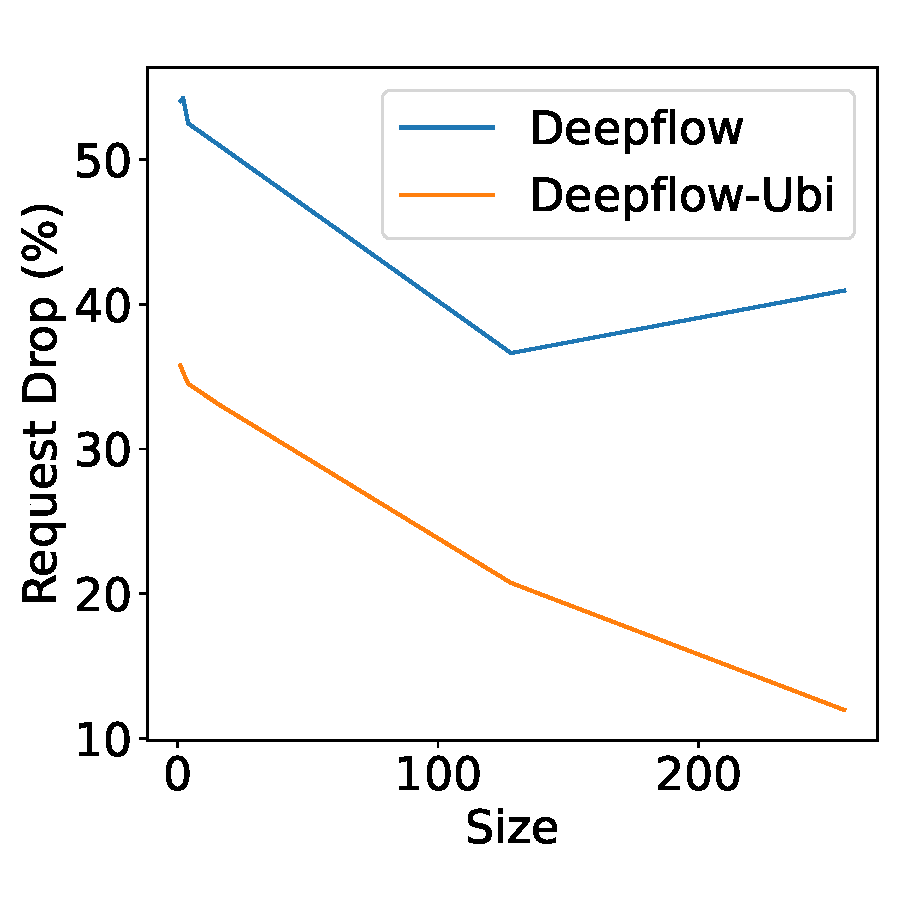
\includegraphics[width=\linewidth]{img/http-request-performance-drop.pdf}
  \caption{HTTPS}
  \label{fig:sub1}
\end{subfigure}%
\begin{subfigure}{.23\textwidth}
  \centering
  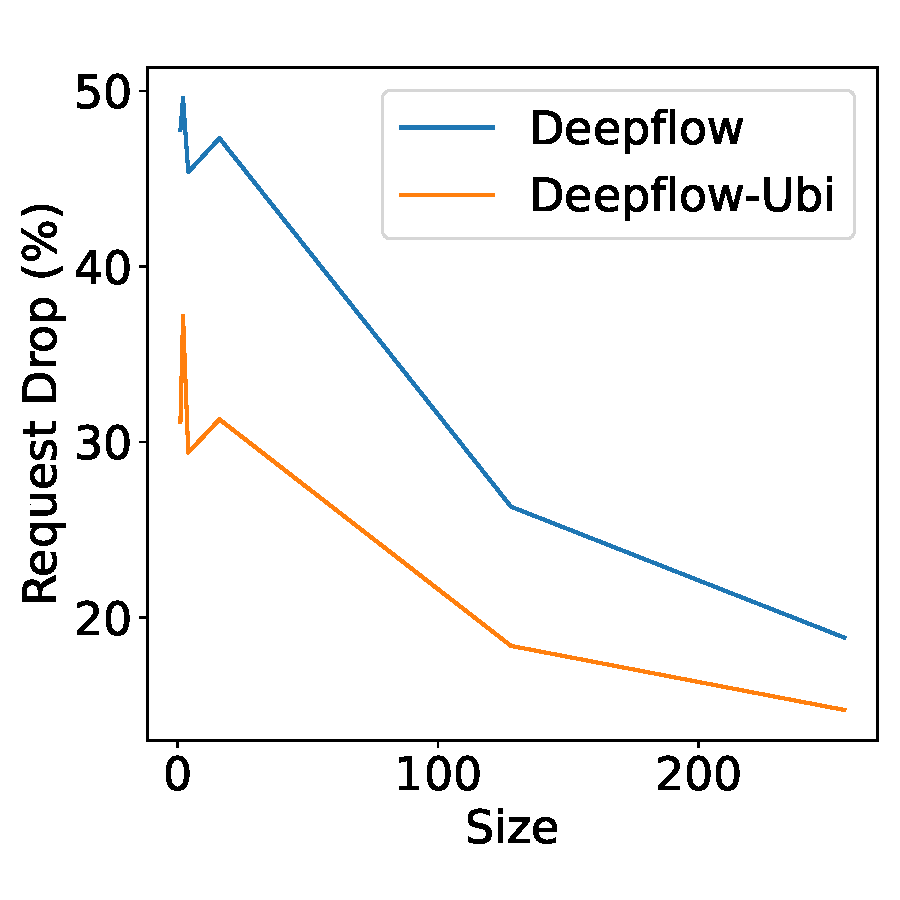
\includegraphics[width=\linewidth]{img/https-request-performance-drop.pdf}
  \caption{HTTP}
  \label{fig:sub2}
\end{subfigure}
\caption{Deepflow throughput overhead}
\label{fig:test}
\end{figure}


We deploy Deepflow on System B and use it to monitor a microservice that returns a random string for each request, implemented on a Golang server and configured to use either HTTP and HTTPS. We route traffic to the service using \texttt{wrk}, configured to use 10 threads with 500 concurrent connections for a 10-second test duration.  We execute the tests with three configurations: native microservice execution without Deepflow, Deepflow using eBPF, and Deepflow using \sys.

We measure the throughput of the microservice as we vary the size of its string response from 1KB to 256KB; \cref{fig:test} shows our results. The native microservice achieves a throughput of between 250,000 requests/second on small keys to 47,000 requests/second on large keys.  DeepFlow using eBPF imposes a significant performance penalty, reducing the throughput of the server by as much as 54\%. \sys reduces this throughput penalty by a factor of 1.5, only reaching a throughput penalty of 36\% in the worst case.

\subsubsection{Durability Tuning}
\begin{figure}[t]
\centering
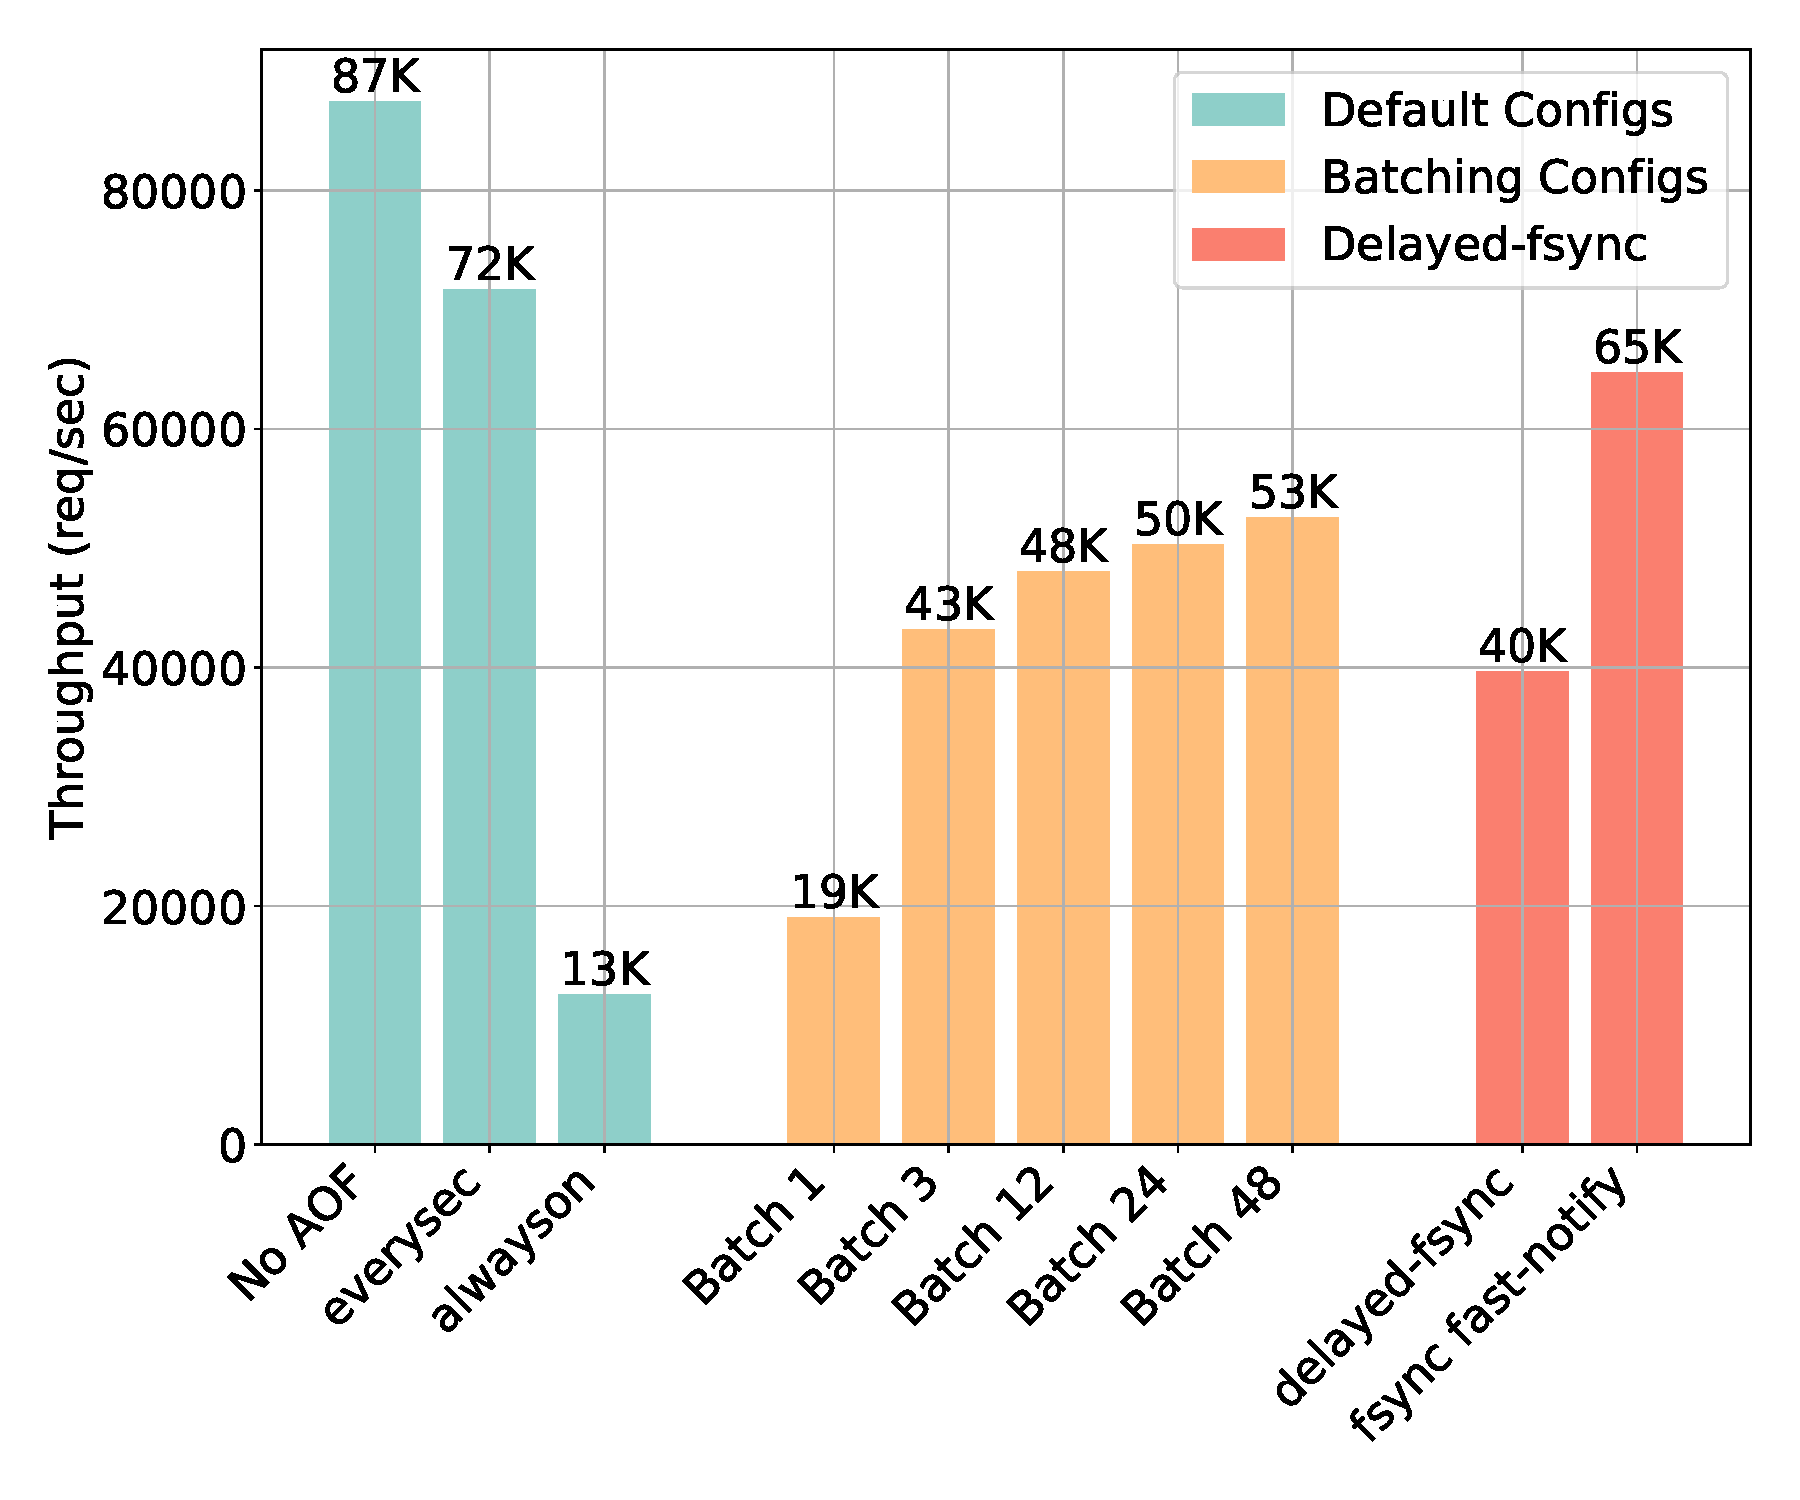
\includegraphics[width=\columnwidth]{img/redis_cluster.pdf}
\caption{Redis throughput with \sys Batch-I/O and Delayed-fsync extensions}\label{fig:redis-batch}
\end{figure}

%\yusheng{we are optimizing the color and layout.}

We evaluate the Durability Tuning use-case on System A and use redis-bench\cite{redis-bench} to send 1M set requests with 5 parallel clients and 3 byte payloads.  We execute redis with the built-in configurations (alwayson, everysec, and No AOF), varied batch sizes (1, 3, 12, 24, and 48), delayed-fsync, and delayed-fsync with the fast-notify optimization.  We configure redis with alwayson when configured to use a batching and delayed-fsync.  \Cref{fig:redis-batch} shows the throughput of each of the configurations.

The batched-I/O exposes interesting durability/performance tradeoffs.  For example, using a batch size of 48 improves redis alwayson throughput by a factor of 4.17, and incurs a modest durability cost of losing ~24 updates in the event (roughly half of the function in a batch are \texttt{write}s).  For comparison, the everysec configuration can lose 72,000 updates in the event of an untimely crash. Thus, a batch size of 48 reduces data loss relative to everysec by three orders of magnitude (2958).  Additionally, we observe that the batched-I/O implementation improves redis performance even for small batches: e.g., a batch size of 1 improves redis alwayson throughput by a factor of 1.51.

Delayed-fsync presents a powerful optimization.  On its own, delayed-fsync achieves a throughput of ~40k requests/second, which is 4.15 times larger than the redis alwayson's throughput. Adding the fast notify user-kernel interaction further accelerates redis to ~65k request/second, more than 5 times larger than redis alwayson.  In sum: delayed-fsync with fast notify is only 10\% slower than redis everysec, but it reduces the number of updates that could be lost in a crash by 5 orders of magnitude (36,000). 

\subsubsection{FUSE}
\begin{table}[t]
\centering
\footnotesize
\begin{tabular}{|l|l|l|}
\hline
\textbf{Test} & \textbf{Native (s)} & \textbf{\sys (s)} \\ \hline \hline
Passthrough, fstat & 3.65 & .176 \\ \hline
LoggedFS, fstat & 7.40 & .184 \\ \hline
LoggedFS, openat& 17.0 & 0.074 \\ \hline
Passthrough, find & 5.1 & 1.6\\\hline
\end{tabular}
\caption{FUSE operation latency.}
\label{tab:fuse}
\end{table}


We evaluate the performance improvement from using \sys to implement caching in FUSE when running on System A.  We deploy two FUSE file systems: Passthrough, which passes filesystem operations to the underlying file system directly, and LoggedFS\cite{loggerFS}, which logs all file system operations to a file before passing them to the underlying file system.  We measure the end-to-end latency of three workloads: one that issues 100000 \texttt{fstatat} calls to a file in the FUSE directory, one that issues 100000 \texttt{openat} calls to a file in the  FUSE directory, and one that uses the linux utility \texttt{find} to travel through the linux 6.7 source code directory.  
%We measure the average single syscall latency for \texttt{fstat} and \texttt{openat}, and measure the end-to-end latency for \texttt{find};   
\Cref{tab:fuse} shows the results on FUSE and with \sys{} caching.  We observe that the caching extension implemented with \sys accelerates the latency of the workloads by a factor of up to four orders of magnitude.
%\arq{I changed these units to seconds and did end-to-end latency rather than average}

\subsubsection{Sslsniff}
\begin{figure}[t]
\centering
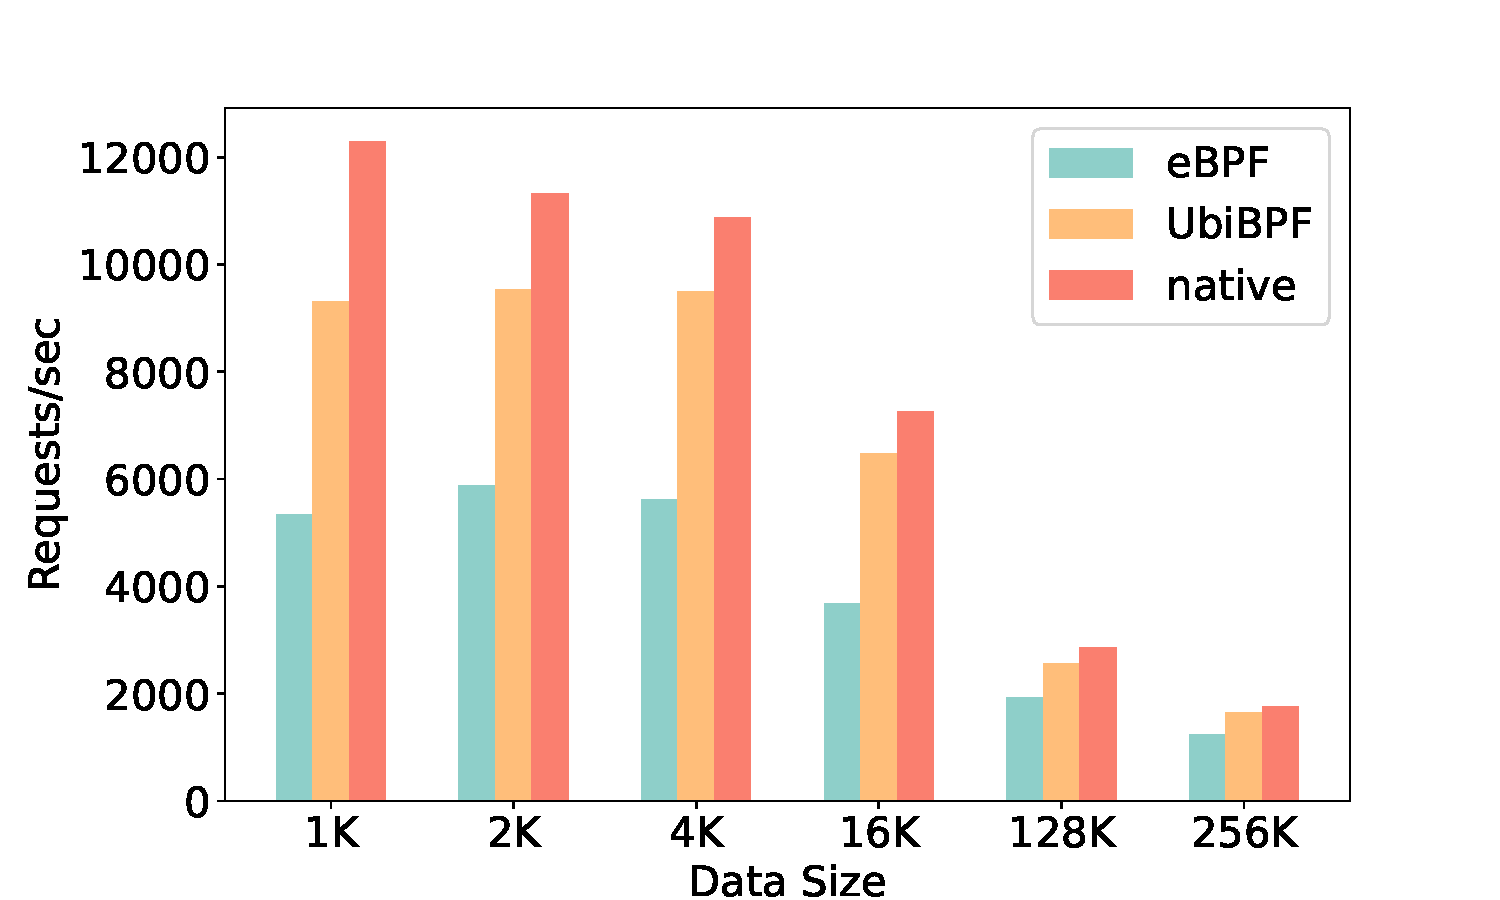
\includegraphics[width=\columnwidth]{img/ssl-nginx.pdf}
\caption{SSlsniff test with nginx}\label{fig:sslsniff}
\end{figure}

We evaluate \texttt{sslsniff} on System B when monitoring  Nginx.  We use the \texttt{wrk} benchmark, configured to use 4 threads with 512 concurrent connections for a 10 second test duration, to generate traffic.   We execute the test on three configurations: native, \texttt{sslsniff} using eBPF, and \texttt{sslsniff} using \sys.  We measure the throughput of Nginx as we vary the response size from 1K to 256KB; \cref{fig:sslsniff} shows the results.  \texttt{sslsniff} using eBPF draastically reduces Nginx performance, reducing throughput compared to native execution by a factor of up to 2.  In contrast, \sys's reduces throughput by a factor of at most 1.2.  

\subsubsection{syscount}

\begin{figure}[t]
\centering
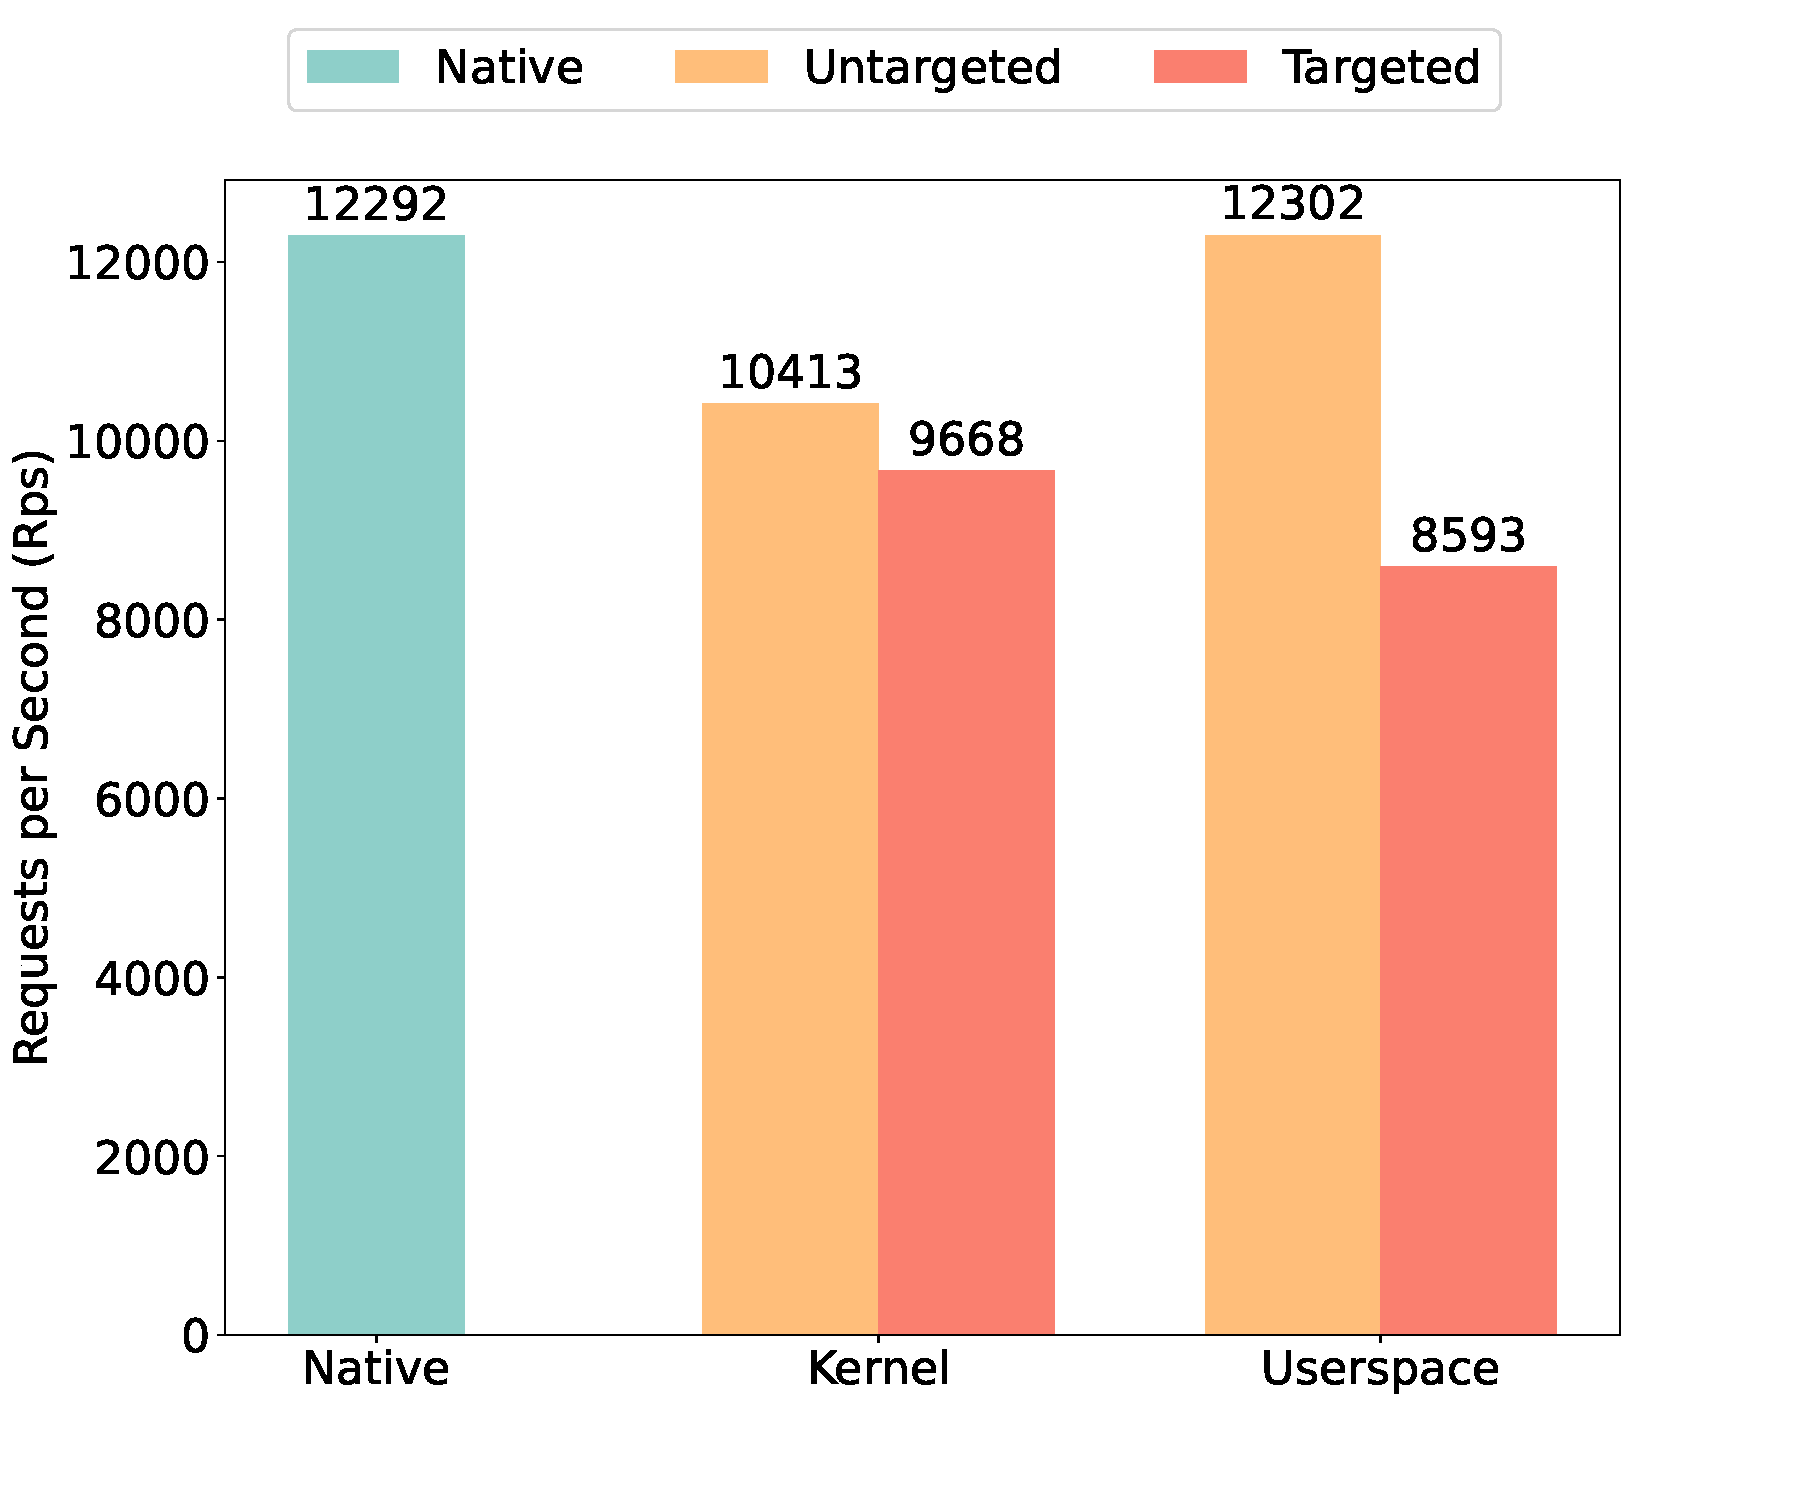
\includegraphics[width=\columnwidth]{img/syscount.pdf}
\caption{syscount test with nginx}\label{fig:sslsniff}
\end{figure}

We evaluate syscount on System B to illustrates the  \sys isolation benefits for monitoring overhead.  We deploy an Nginx server and route traffic to the server using the \texttt{wrk} benchmark, configured to use 4 threads with 512 concurrent connections for a 10-second test duration.  We measure the throughput of Nginx in five tests: (1) native Nginx, (2) syscount on the Nginx process using a kernel eBPF extension, (3) syscount on a different process using a kernel eBPF extension, (4) syscount on the Nginx process using a \sys{} userspace extension, and (5) syscount on a different process using a \sys{} userspace extension. \Cref{fig:sslsniff} shows the throughput of each of the configurations. We observe that user-mode systemcall tracing incurs more overhead than eBPF: the throughput drop from using kernel extensions is only 21.35\%, but the throughput drop from using user-mode \sys extensions is 30.09\%.  However, we also observe isolation benefits from \sys: the throughput drop from using kernel extension to monitor a different process is 15.29\%, but the throughput is not effected when using userspace \sys extension to monitor a different process. 

%\arq{Let's fix this graph!  As presented its pretty confusing, it's also missing some data. It should be a clustered bar chart.  The cluster all the way on the left shows native execution (labeled native).  The next cluster includes two bars, both of which are using kernel probes.  The first bar shows the overhead on Nginx when it is being monitored, the second bar shows the overhead of Nginx when another process is monitored.  The final cluster includes two bars, both of which are \sys.  The first bar shows the overhead on Nginx when it is moniotred with \sys, the second bar shows the overhead of Nginx when another process is monitored with \sys.} Good job

\subsubsection{Nginx Plugin}

\begin{table}[t]
\centering
\footnotesize
\begin{tabular}{|l|c|c|}
\hline
\textbf{Configuration}       & \textbf{Througput} & \textbf{Overhead} \\ \hline\hline
Native & 147000             & -               \\ \hline
\sys security    & 135000             & 8 \%              \\ \hline
Lua security   & 114000             & 22 \%              \\ \hline
Wasm security  & 106000             & 28 \%             \\ \hline
\end{tabular}
\caption{Comparison of extension approaches for Nginx}
\label{tab:nginx-plugin}
\end{table}

We evaluate the performance improvement from using \sys to extend Nginx compared to current Nginx plugins.  We deploy the security module and a tracing module in a Nginx running on System B and use \texttt{wrk} configured to use 10 worker threads with 100 concurrent connections and target a test time of 10s. We compare native Nginx execution to the security module written using \sys{} and the security module written using Nginx's Lua and WebAssembly plugins. \Cref{tab:nginx-plugin} shows the throughput of each of the configurations. \sys's extension results in an 8\% overhead compared to no filtering, whereas Lua and Wasm incur a 22\% and 28\% overhead, respectively.  Thus, \sys has 2.75x and 3.5x less overhead than Lua and Wasm.

\subsection{Microbenchmark Performance}
\begin{figure*}[t]
\centering
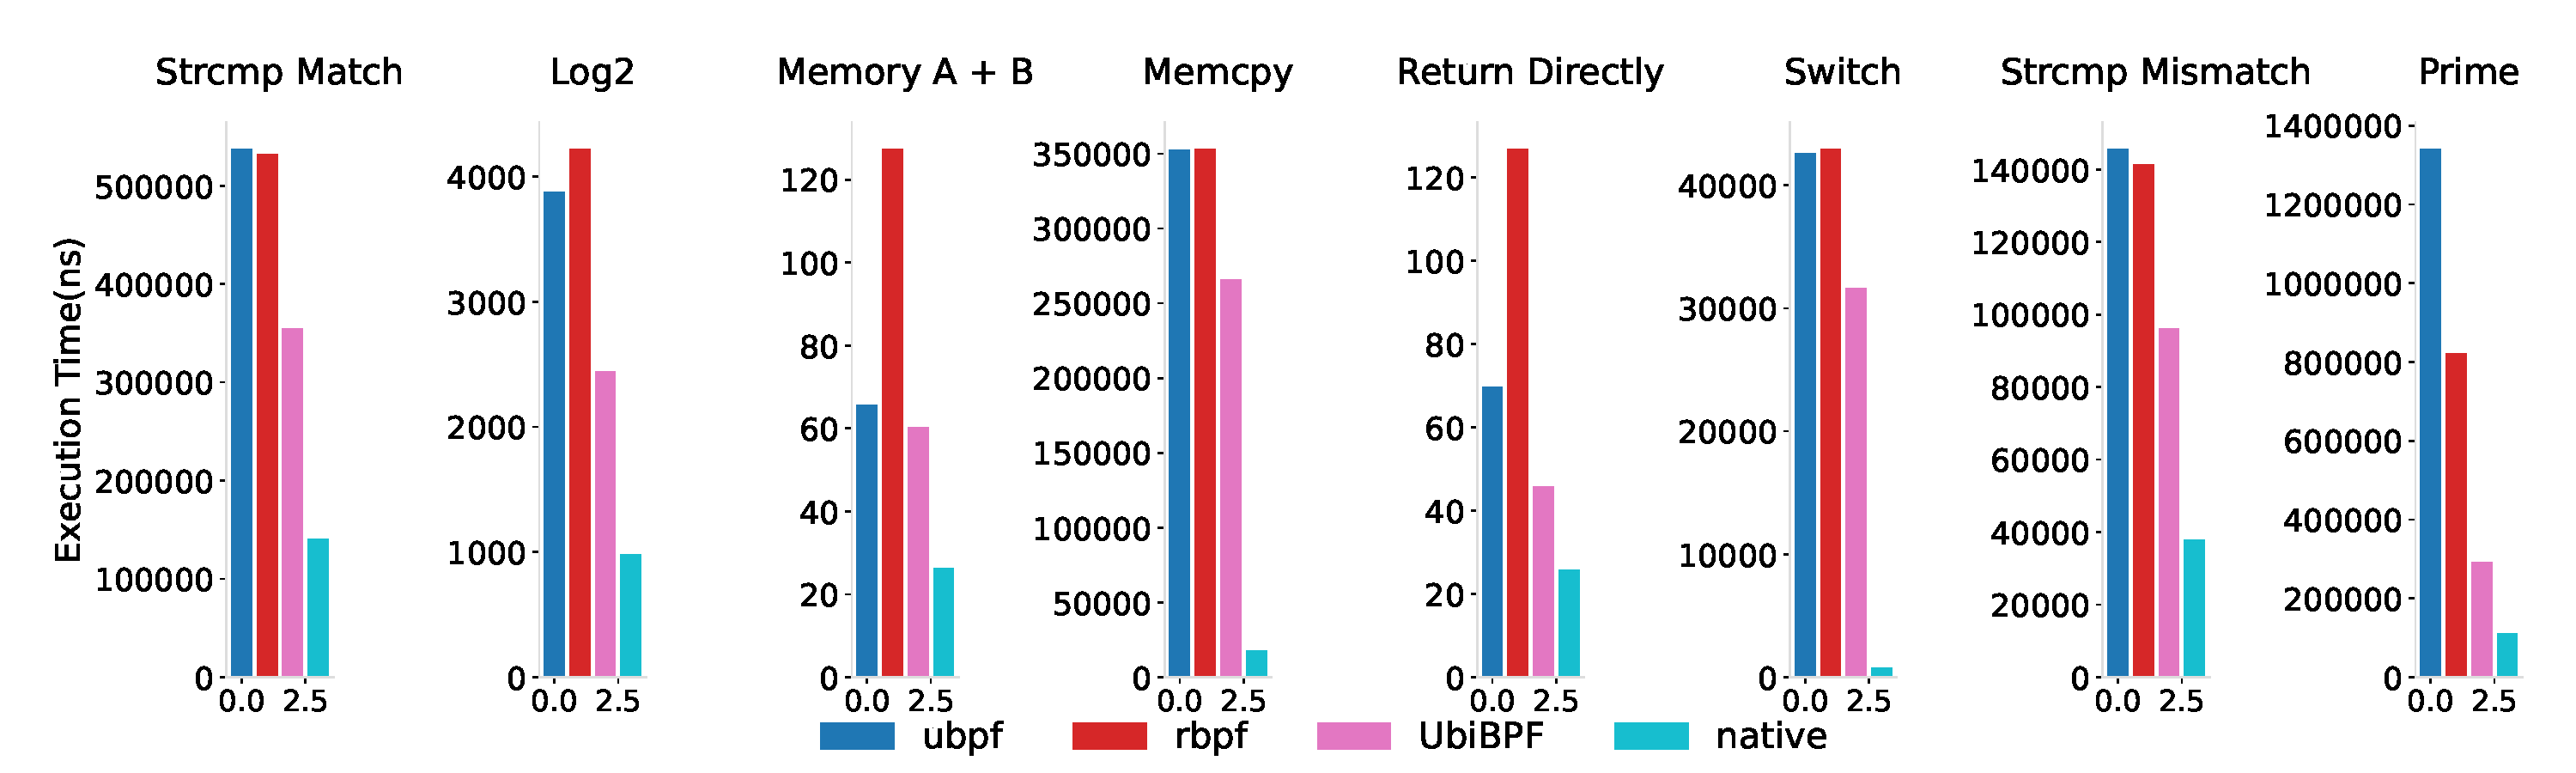
\includegraphics[width=\textwidth]{img/jit_execution_times.pdf}
\caption{Performance comparison of \sys, ubpf, rbpf, and native on microbenchmarks. \label{fig:uvm}}
\end{figure*}

We use microbenchmarks to explore \sys's efficiency.  In summary, we show that \sys's superiority comes from low per-probe latency and an efficient  eBPF bytecode execution.

\subsubsection{Probe Performance}
\begin{table}[t]
\footnotesize

    \centering
    \begin{tabular}{|c|c|c|}
        \hline
        \textbf{Probe Type} & \textbf{eBPF} (ns) & \textbf{\sys} (ns)\\
        \hline\hline
        Uprobe & 3224 & 315 \\
        Uretprobe & 3997 & 381\\
        Syscall Tracepoint & 152 & 233\\
        \hline
    \end{tabular}
    \caption{Microbenchmark comparison of \sys and eBPF.}
    \label{tab:probe_comparison}
\end{table}

We create microbenchmarks that inject and then repeatedly execute a no-op \texttt{uprobe}, \texttt{uretprobe}, and \texttt{syscall tracepoint} and execute them on system A.   \Cref{tab:probe_comparison} shows the latency of each of the probe types on eBPF and \sys.  We observe that \sys is more than an order of magnitude faster than eBPF at executing \texttt{uprobe} and \texttt{uretprobe}s, but 1.5 times slower at executing \texttt{syscall tracepoint}s.  To determine an ideal probe overhead, we statically instrument a function in our benchmark with a no-op function and observe its latency as 110 ns.  Thus, \sys's \texttt{uprobe} and \texttt{uretprobe} latencies are only a few hundred ns slower than the ideal latency. 

\subsubsection{\sys execution engine efficiency}

We evaluate the efficiency of our \sys JIT component compared to ubpf and rbpf, existing userspace eBPF virtual machines.  We write 8 micro-benchmarks, include integer heavy computation (`log2', `prime'), memory heavy workloads (`memory a+b', `memcpy'), cstring benchmarks (`strcmp match', `strcmp mismatch'), and control-flow benchmarks (`return directly', `switch').  \Cref{fig:uvm} shows the latency of each microbenchmark.  We observe that \sys is a significant improvement compared to existing eBPF runtimes (ubpf and rbpf), accelerating average benchmark latency by a factor of 1.53 and 1.72 compared to ubpf and rbpf, respectively. 

%\yusheng{9.05 is the avg of factors, it's because in memcpy and switch, native is much faster than others. 3.38 is summary all usecases, so I think we don't need to mention it here, it's hard to calc because we have so me=any different benches here.}
%3.38 mainly comes from the start and isolation delay of vm. and also the strcmp in native is using some hardware instructions to spend up.

%\arq{This graph needs a bit of help. Remove the `-jit' from ubpf and rbpf. Remove WASM from the graph (it is not helpful for the reader), and replable "<NATIVE>" to "native".  Calculate the overheads that I asked for above (the xyzs)} \arq{perfect!}

\subsubsection{\sys Load latency}
We evaluate the latency of loading an extension with \sys.  We write a test that monitors \texttt{malloc} in \texttt{libc} and measure \sys's loading latency. We load the extension into a running process and observe a 48ms load latency.  For comparison, we load the same extension using LD\_PRELOAD, a conventional technique for extending software, and observe a 30ms load latency.

\subsection{\sys Compatibility}
\begin{comment}
\begin{table}[t]
    \centering
    \begin{tabular}{|c|c|c|c|}
        \hline
        \textbf{eBPF linux} & \textbf{ubpf} & \textbf{rbpf} & \textbf{\sys} \\
        \hline\hline
        166/166 & 144/166 & 143/166 & 165/166 \\
        \hline
    \end{tabular}
    \caption{eBPF JIT pass conformance tests.}
    \label{tab:conformance}
\end{table}
\end{comment}

We evaluate the compatibility of \sys with existing eBPF full-system extensions. \sys works on all of the 17 BCC~\cite{bcc} and bpftrace~\cite{bpftrace} tools.  Also, \sys{} fails only one test in the the bpf-conformance test suite~\cite{bpfconformance}, whereas ubpf and rbpf fail 22 and 23, respectively.
% \input{discuss}
\section{Related Work}\label{sec:related_work}
% go back
\sys is the first system to support comprehensive, safe, dynamic, and efficient extensions. 

Many systems support software customization through an extension primitive allowing developers to observe or modify a system's default behavior.  Nearly all existing work supports extending either an operating system kernel (\eg Nooks~\cite{Swift03}, VINO~\cite{Seltzer96}, SPIN~\cite{Bershad95}) or an application (\eg PIN~\cite{Luk05}, Valgrind~\cite{Nethercote07}, DynamoRIO~\cite{Bruening12}).  In contrast to these systems, \sys supports comprehensive extensions---\ie ones that extend both userspace applications and a kernel.

eBPF is the de facto extension framework in linux and has recently been adopted in Windows~\cite {eBPFWindows}.  eBPF is \emph{almost} comprehensive, except that eBPF userspace extensions cannot modify application behavior.  Moreover, eBPF's appraoch to safety executes userspace extensions in the kernel which comes with high overhead.  \sys{} resolves the comprehensiveness and efficiency issues of eBPF by executing userspace extensions directly in the execution context of the target application without requiring kernel involvement.

Ensuring system safety in the presence of software extensions requires isolating extension logic from the original logic of the program.  Many systems isolate untrusted extension code in a sandbox through the use of software fault isolation (SFI)~\cite{Wahbe93}.  For example,  dynamic instrumentation frameworks~\cite{Luk05, Nethercote07, Bruening12}, and lightweight virtual machines (\eg WebAssembly~\cite{webassembly}, NaCL~\cite{Yee09}, RLBox~\cite{Narayan20}), execute programs in a virtualized environment that monitors all memory and control-flow operations to isolate failures.  These approaches impose a high runtime overhead that precludes efficiency.

\sys{}'s use of intra-process memory protections is adopted from the approaches taken by Donky~\cite{schrammel2020donky}, ERIM~\cite{Vahldiek19} and libmpk~\cite{Park19}.  \sys{}'s key differences between these systems is the target domain---\sys{} applies these ideas to extend an existing application without requiring source-code changes, whereas prior work uses intra-process memory protection to provide lightweight protection domains that a rewritten application can use. There are many lightweight isolation abstractions that have been proposed (\eg Wedge~\cite{Bittau08}, Lightweight contexts~\cite{Litton16}, Orbit~\cite{Jing22}, \etc); \sys{} differs from these works in its target domain.

ubpf~\cite{ubpf} and rbpf~\cite{rbpf} implement virtual machines for executing eBPF bytecode in userspace.  These systems have higher runtime overhead compared to \sys's runtime that uses LLVM's ORC JIT\cite{Lattner04,lu2022bring} (see \cref{sec:design}).  Additionally, ubpf and rbpf are incomplete in that they do not support as many eBPF features as \sys and do not support eBPF Maps.

%\yusheng{
%The ubpf uses handwritten single pass jit, without doing much optimization. The rbpf is using cranelift JIT, and \sys is using LLVM jit. The \sys jit is faster thanks to the optimization from LLVM. We lift the bpf bytecode to llvm bytecode, and config llvm passes to optimize it.(Try to maximize the optimization level). The performance evaluation can be provided.

%Also, they doesn't support as many eBPF features as \sys. For example, they doesn't support atomic eBPF instructions.We have a conformance test for it, many we can put the compare in evaluation?

%This is for the eBPF virtual machine, but I think the most difference between the \sys and ubpf/rbpf is that they doesn't support eBPF maps in share memory or in kernel, and they cannot attach to userspace functions or syscalls, also they cannot dynamically inject in to a running process. They are just virtual machines.} \arq{thanks!}

\begin{comment}

\subsection{Dynamic Binary Instrumentation}

Dynamic Binary Instrumentation (DBI) facilitates real-time analysis of binary applications by injecting instrumentation code during runtime. This mechanism permits the embedding of specific analysis code into a program as it executes, tailored to user specifications, without disrupting the dynamic execution flow of the program. Renowned platforms that provide dynamic binary analysis capabilities include Pin\cite{1550984}, DynamoRIO\cite{dynamorio}, and Frida\cite{fridagum}. The defining attributes of DBI encompass its capability to work directly on binary code, obviating the need for source code, and its dynamic modus operandi which allows on-the-fly modifications to the program, thus negating the necessity for recompilation or program restarts. Nonetheless, DBI comes with certain caveats: it lacks built-in security checks or verification measures which may pose potential security risks. Moreover, in the absence of a high-performance virtual machine (VM) and an encapsulated sandbox environment, the efficiency of DBI could be compromised, and there's a potential to disrupt the execution states of the target process. Furthermore, existing DBI tools fall short in providing a high-performance control panel or data aggregation mechanisms akin to the capabilities offered by eBPF maps.

\subsection{WebAssembly}

WebAssembly (Wasm)\cite{webassembly} is a binary instruction format created as a portable compilation target for high-level languages such as C, C++, and Rust. It endeavors to achieve execution at native speed by leveraging common hardware capabilities. WebAssembly's design ensures portability across all modern platforms, both on desktop and mobile. It also operates within a sandboxed execution environment to maintain secure execution. With its binary format, WebAssembly enables faster parsing, compiling, and execution compared to traditional text-based web technologies. The structure and principles behind WebAssembly make it a suitable platform for various use cases beyond the web, including blockchain, serverless computing, and portable CLI tools, among others.

Both Dynamic Binary Instrumentation and WebAssembly illustrate unique approaches to runtime code analysis and execution. While DBI offers detailed insights into binary code behavior during runtime, WebAssembly provides a secure and portable compilation target. The exploration of these technologies, alongside the development of \textit{bpftime}, contributes to the broader effort of advancing runtime code analysis and execution frameworks.

\end{comment}
\section{Conclusion}\label{sec:conclusion}

In this work, we presented \sys, a comprehensive, dynamic, safe, and efficient extension framework. \sys is based upon two design principles: maintaining compatibility with the existing eBPF ecosystem and executing userspace extensions in the extended application without requiring kernel involvement.  We show that \sys full system extensions are useful across \numcases case studies and that the system provides a large performance improvement compared to existing state-of-the-art full system extension tools.  We  will release \sys as an open-source project. 

%, a cutting-edge userspace eBPF runtime designed to alleviate the identified performance and security drawbacks inherent to kernel eBPF. Through \textit{bpftime}, we significantly improved Uprobe and Syscall hook performance, demonstrating a tenfold reduction in Uprobe overhead relative to kernel uprobes. Our runtime showcases a smooth integration with ongoing processes, bypassing the need for restarts or manual recompilations. Compatibility with prevalent eBPF toolchains like clang and libbpf simplifies userspace eBPF development, portraying \textit{bpftime} as a step forward in enhancing userspace eBPF runtimes. The open-sourced nature of \textit{bpftime} at \href{https://github.com/eunomia-bpf/bpftime}{https://github.com/eunomia-bpf/bpftime} paves the way for community engagement, fostering further exploration and innovation in this domain.

\bibliographystyle{plain}
\bibliography{cite}

\end{document}